\documentclass[twoside]{book}

% Packages required by doxygen
\usepackage{fixltx2e}
\usepackage{calc}
\usepackage{doxygen}
\usepackage{graphicx}
\usepackage[utf8]{inputenc}
\usepackage{makeidx}
\usepackage{multicol}
\usepackage{multirow}
\PassOptionsToPackage{warn}{textcomp}
\usepackage{textcomp}
\usepackage[nointegrals]{wasysym}
\usepackage[table]{xcolor}

% Font selection
\usepackage[T1]{fontenc}
\usepackage{mathptmx}
\usepackage[scaled=.90]{helvet}
\usepackage{courier}
\usepackage{amssymb}
\usepackage{sectsty}
\renewcommand{\familydefault}{\sfdefault}
\allsectionsfont{%
  \fontseries{bc}\selectfont%
  \color{darkgray}%
}
\renewcommand{\DoxyLabelFont}{%
  \fontseries{bc}\selectfont%
  \color{darkgray}%
}
\newcommand{\+}{\discretionary{\mbox{\scriptsize$\hookleftarrow$}}{}{}}

% Page & text layout
\usepackage{geometry}
\geometry{%
  a4paper,%
  top=2.5cm,%
  bottom=2.5cm,%
  left=2.5cm,%
  right=2.5cm%
}
\tolerance=750
\hfuzz=15pt
\hbadness=750
\setlength{\emergencystretch}{15pt}
\setlength{\parindent}{0cm}
\setlength{\parskip}{0.2cm}
\makeatletter
\renewcommand{\paragraph}{%
  \@startsection{paragraph}{4}{0ex}{-1.0ex}{1.0ex}{%
    \normalfont\normalsize\bfseries\SS@parafont%
  }%
}
\renewcommand{\subparagraph}{%
  \@startsection{subparagraph}{5}{0ex}{-1.0ex}{1.0ex}{%
    \normalfont\normalsize\bfseries\SS@subparafont%
  }%
}
\makeatother

% Headers & footers
\usepackage{fancyhdr}
\pagestyle{fancyplain}
\fancyhead[LE]{\fancyplain{}{\bfseries\thepage}}
\fancyhead[CE]{\fancyplain{}{}}
\fancyhead[RE]{\fancyplain{}{\bfseries\leftmark}}
\fancyhead[LO]{\fancyplain{}{\bfseries\rightmark}}
\fancyhead[CO]{\fancyplain{}{}}
\fancyhead[RO]{\fancyplain{}{\bfseries\thepage}}
\fancyfoot[LE]{\fancyplain{}{}}
\fancyfoot[CE]{\fancyplain{}{}}
\fancyfoot[RE]{\fancyplain{}{\bfseries\scriptsize Generated on Mon Nov 14 2016 20\+:11\+:37 for tp\+\_\+inf224 by Doxygen }}
\fancyfoot[LO]{\fancyplain{}{\bfseries\scriptsize Generated on Mon Nov 14 2016 20\+:11\+:37 for tp\+\_\+inf224 by Doxygen }}
\fancyfoot[CO]{\fancyplain{}{}}
\fancyfoot[RO]{\fancyplain{}{}}
\renewcommand{\footrulewidth}{0.4pt}
\renewcommand{\chaptermark}[1]{%
  \markboth{#1}{}%
}
\renewcommand{\sectionmark}[1]{%
  \markright{\thesection\ #1}%
}

% Indices & bibliography
\usepackage{natbib}
\usepackage[titles]{tocloft}
\setcounter{tocdepth}{3}
\setcounter{secnumdepth}{5}
\makeindex

% Hyperlinks (required, but should be loaded last)
\usepackage{ifpdf}
\ifpdf
  \usepackage[pdftex,pagebackref=true]{hyperref}
\else
  \usepackage[ps2pdf,pagebackref=true]{hyperref}
\fi
\hypersetup{%
  colorlinks=true,%
  linkcolor=blue,%
  citecolor=blue,%
  unicode%
}

% Custom commands
\newcommand{\clearemptydoublepage}{%
  \newpage{\pagestyle{empty}\cleardoublepage}%
}


%===== C O N T E N T S =====

\begin{document}

% Titlepage & ToC
\hypersetup{pageanchor=false,
             bookmarks=true,
             bookmarksnumbered=true,
             pdfencoding=unicode
            }
\pagenumbering{roman}
\begin{titlepage}
\vspace*{7cm}
\begin{center}%
{\Large tp\+\_\+inf224 }\\
\vspace*{1cm}
{\large Generated by Doxygen 1.8.8}\\
\vspace*{0.5cm}
{\small Mon Nov 14 2016 20:11:37}\\
\end{center}
\end{titlepage}
\clearemptydoublepage
\tableofcontents
\clearemptydoublepage
\pagenumbering{arabic}
\hypersetup{pageanchor=true}

%--- Begin generated contents ---
\chapter{Hierarchical Index}
\section{Class Hierarchy}
This inheritance list is sorted roughly, but not completely, alphabetically\+:\begin{DoxyCompactList}
\item \contentsline{section}{cppu\+:\+:T\+C\+P\+Server\+:\+:Callback}{\pageref{structcppu_1_1_t_c_p_server_1_1_callback}}{}
\begin{DoxyCompactList}
\item \contentsline{section}{cppu\+:\+:T\+C\+P\+Server\+:\+:Callback\+Method$<$ T $>$}{\pageref{structcppu_1_1_t_c_p_server_1_1_callback_method}}{}
\end{DoxyCompactList}
\item \contentsline{section}{Fabriquer}{\pageref{class_fabriquer}}{}
\item \contentsline{section}{cppu\+:\+:Input\+Buffer}{\pageref{structcppu_1_1_input_buffer}}{}
\item list\begin{DoxyCompactList}
\item \contentsline{section}{Groupe}{\pageref{class_groupe}}{}
\end{DoxyCompactList}
\item \contentsline{section}{Omultimedia}{\pageref{class_omultimedia}}{}
\begin{DoxyCompactList}
\item \contentsline{section}{Photo}{\pageref{class_photo}}{}
\item \contentsline{section}{Video}{\pageref{class_video}}{}
\begin{DoxyCompactList}
\item \contentsline{section}{Film}{\pageref{class_film}}{}
\end{DoxyCompactList}
\end{DoxyCompactList}
\item \contentsline{section}{cppu\+:\+:Server\+Socket}{\pageref{classcppu_1_1_server_socket}}{}
\item \contentsline{section}{cppu\+:\+:Socket}{\pageref{classcppu_1_1_socket}}{}
\item \contentsline{section}{cppu\+:\+:Socket\+Buffer}{\pageref{classcppu_1_1_socket_buffer}}{}
\begin{DoxyCompactList}
\item \contentsline{section}{cppu\+:\+:T\+C\+P\+Connection}{\pageref{classcppu_1_1_t_c_p_connection}}{}
\end{DoxyCompactList}
\item \contentsline{section}{cppu\+:\+:T\+C\+P\+Lock}{\pageref{classcppu_1_1_t_c_p_lock}}{}
\item \contentsline{section}{cppu\+:\+:T\+C\+P\+Server}{\pageref{classcppu_1_1_t_c_p_server}}{}
\end{DoxyCompactList}

\chapter{Class Index}
\section{Class List}
Here are the classes, structs, unions and interfaces with brief descriptions\+:\begin{DoxyCompactList}
\item\contentsline{section}{\hyperlink{structcppu_1_1_t_c_p_server_1_1_callback}{cppu\+::\+T\+C\+P\+Server\+::\+Callback} \\*\hyperlink{structcppu_1_1_t_c_p_server_1_1_callback}{Callback} interface }{\pageref{structcppu_1_1_t_c_p_server_1_1_callback}}{}
\item\contentsline{section}{\hyperlink{structcppu_1_1_t_c_p_server_1_1_callback_method}{cppu\+::\+T\+C\+P\+Server\+::\+Callback\+Method$<$ T $>$} }{\pageref{structcppu_1_1_t_c_p_server_1_1_callback_method}}{}
\item\contentsline{section}{\hyperlink{class_fabriquer}{Fabriquer} }{\pageref{class_fabriquer}}{}
\item\contentsline{section}{\hyperlink{class_film}{Film} }{\pageref{class_film}}{}
\item\contentsline{section}{\hyperlink{class_groupe}{Groupe} }{\pageref{class_groupe}}{}
\item\contentsline{section}{\hyperlink{structcppu_1_1_input_buffer}{cppu\+::\+Input\+Buffer} }{\pageref{structcppu_1_1_input_buffer}}{}
\item\contentsline{section}{\hyperlink{class_my_base}{My\+Base} }{\pageref{class_my_base}}{}
\item\contentsline{section}{\hyperlink{class_omultimedia}{Omultimedia} }{\pageref{class_omultimedia}}{}
\item\contentsline{section}{\hyperlink{class_photo}{Photo} }{\pageref{class_photo}}{}
\item\contentsline{section}{\hyperlink{classcppu_1_1_server_socket}{cppu\+::\+Server\+Socket} \\*T\+C\+P/\+I\+P server socket. This class implements a T\+C\+P/\+I\+P socket that waits for requests to come in over the network. A\+F\+\_\+\+I\+N\+E\+T connections following the I\+Pv4 Internet protocol are supported }{\pageref{classcppu_1_1_server_socket}}{}
\item\contentsline{section}{\hyperlink{classcppu_1_1_socket}{cppu\+::\+Socket} \\*T\+C\+P/\+I\+P or U\+D\+P/\+Datagram socket. This class encapsulates a T\+C\+P/\+I\+P or U\+D\+P/\+Datagram socket. A\+F\+\_\+\+I\+N\+E\+T connections following the I\+Pv4 Internet protocol are supported }{\pageref{classcppu_1_1_socket}}{}
\item\contentsline{section}{\hyperlink{classcppu_1_1_socket_buffer}{cppu\+::\+Socket\+Buffer} \\*Preserves record boundaries when exchanging data between connected T\+C\+P/\+I\+P sockets. This class ensures that one call to \hyperlink{classcppu_1_1_socket_buffer_a92ae0351aaee8719d34e8c4618495d59}{write\+Line()} corresponds to one and exactly one call to \hyperlink{classcppu_1_1_socket_buffer_a222769d3776b9cbd3a727ee1f0e60358}{read\+Line()} on the other side. This differs from the behavior of \hyperlink{classcppu_1_1_socket_aeac77f859159715e2d63a5a0dc118788}{Socket\+::send()} and \hyperlink{classcppu_1_1_socket_a37c382af52cc02f92c0e19a0c6e0e04f}{Socket\+::receive()} because T\+C\+P/\+I\+P connected sockets do not preserve record boundaries. \hyperlink{classcppu_1_1_socket_buffer_a92ae0351aaee8719d34e8c4618495d59}{write\+Line()} and \hyperlink{classcppu_1_1_socket_buffer_a222769d3776b9cbd3a727ee1f0e60358}{read\+Line()} solve this problem by automatically adding and searching for a separator between successive lines }{\pageref{classcppu_1_1_socket_buffer}}{}
\item\contentsline{section}{\hyperlink{classcppu_1_1_t_c_p_connection}{cppu\+::\+T\+C\+P\+Connection} \\*Connection with a given client. Each \hyperlink{classcppu_1_1_t_c_p_connection}{T\+C\+P\+Connection} uses a different thread }{\pageref{classcppu_1_1_t_c_p_connection}}{}
\item\contentsline{section}{\hyperlink{classcppu_1_1_t_c_p_lock}{cppu\+::\+T\+C\+P\+Lock} \\*Locks the server in read mode or in write mode. Must be created {\itshape in the stack} by the callback method }{\pageref{classcppu_1_1_t_c_p_lock}}{}
\item\contentsline{section}{\hyperlink{classcppu_1_1_t_c_p_server}{cppu\+::\+T\+C\+P\+Server} \\*T\+C\+P/\+I\+P I\+Pv4 server. The server supports T\+C\+P/\+I\+P A\+F\+\_\+\+I\+N\+E\+T connections (following the I\+Pv4 Internet protocol) with multiple clients. One thread is used per client }{\pageref{classcppu_1_1_t_c_p_server}}{}
\item\contentsline{section}{\hyperlink{class_video}{Video} }{\pageref{class_video}}{}
\end{DoxyCompactList}

\chapter{Class Documentation}
\hypertarget{structcppu_1_1_t_c_p_server_1_1_callback}{\section{cppu\+:\+:T\+C\+P\+Server\+:\+:Callback Struct Reference}
\label{structcppu_1_1_t_c_p_server_1_1_callback}\index{cppu\+::\+T\+C\+P\+Server\+::\+Callback@{cppu\+::\+T\+C\+P\+Server\+::\+Callback}}
}


\hyperlink{structcppu_1_1_t_c_p_server_1_1_callback}{Callback} interface.  




{\ttfamily \#include $<$tcpserver.\+h$>$}



Inheritance diagram for cppu\+:\+:T\+C\+P\+Server\+:\+:Callback\+:
\nopagebreak
\begin{figure}[H]
\begin{center}
\leavevmode
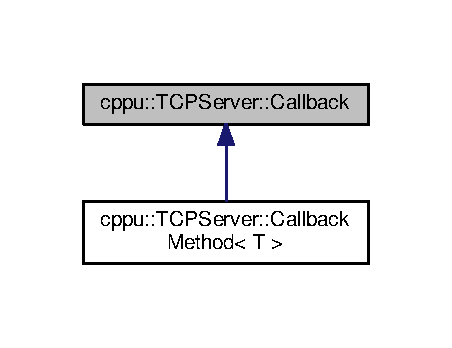
\includegraphics[width=217pt]{structcppu_1_1_t_c_p_server_1_1_callback__inherit__graph}
\end{center}
\end{figure}
\subsection*{Public Member Functions}
\begin{DoxyCompactItemize}
\item 
\hypertarget{structcppu_1_1_t_c_p_server_1_1_callback_aabe4b0b30e14ddeb7c0c02aa3a335eba}{virtual bool {\bfseries call} (\hyperlink{classcppu_1_1_t_c_p_connection}{T\+C\+P\+Connection} \&cnx, const std\+::string \&request, std\+::string \&response)=0}\label{structcppu_1_1_t_c_p_server_1_1_callback_aabe4b0b30e14ddeb7c0c02aa3a335eba}

\end{DoxyCompactItemize}


\subsection{Detailed Description}
\hyperlink{structcppu_1_1_t_c_p_server_1_1_callback}{Callback} interface. 

The documentation for this struct was generated from the following file\+:\begin{DoxyCompactItemize}
\item 
/cal/homes/fouotsap/\+Desktop/\+Fouotsap\+\_\+\+Foukmeniok\+\_\+\+Alain/cpp/tcpserver.\+h\end{DoxyCompactItemize}

\hypertarget{structcppu_1_1_t_c_p_server_1_1_callback_method}{\section{cppu\+:\+:T\+C\+P\+Server\+:\+:Callback\+Method$<$ T $>$ Struct Template Reference}
\label{structcppu_1_1_t_c_p_server_1_1_callback_method}\index{cppu\+::\+T\+C\+P\+Server\+::\+Callback\+Method$<$ T $>$@{cppu\+::\+T\+C\+P\+Server\+::\+Callback\+Method$<$ T $>$}}
}


Inheritance diagram for cppu\+:\+:T\+C\+P\+Server\+:\+:Callback\+Method$<$ T $>$\+:
\nopagebreak
\begin{figure}[H]
\begin{center}
\leavevmode
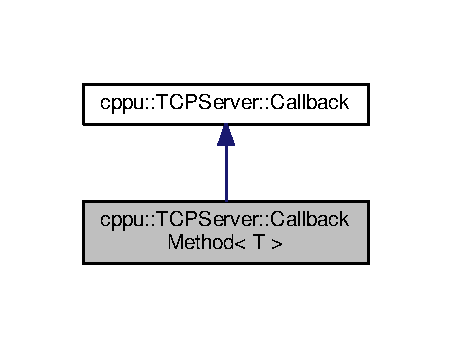
\includegraphics[width=217pt]{structcppu_1_1_t_c_p_server_1_1_callback_method__inherit__graph}
\end{center}
\end{figure}


Collaboration diagram for cppu\+:\+:T\+C\+P\+Server\+:\+:Callback\+Method$<$ T $>$\+:
\nopagebreak
\begin{figure}[H]
\begin{center}
\leavevmode
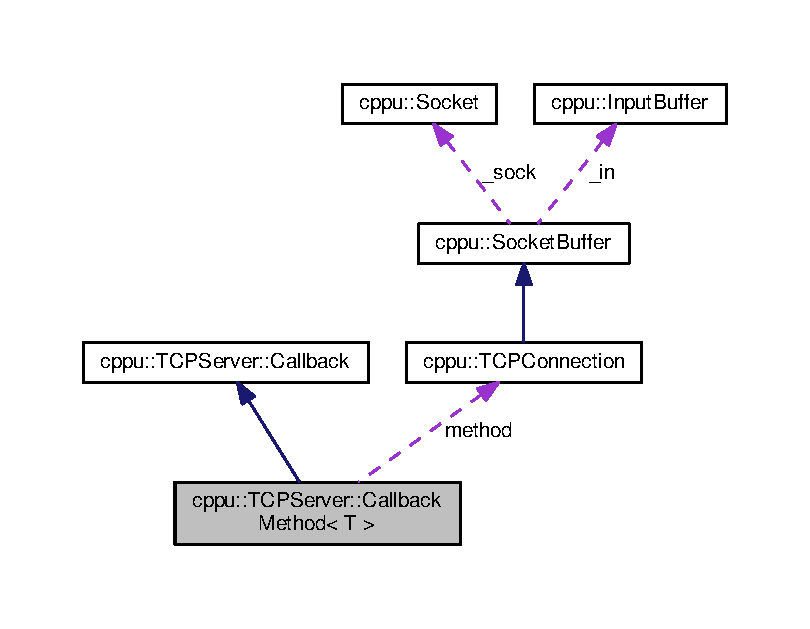
\includegraphics[width=350pt]{structcppu_1_1_t_c_p_server_1_1_callback_method__coll__graph}
\end{center}
\end{figure}
\subsection*{Public Types}
\begin{DoxyCompactItemize}
\item 
\hypertarget{structcppu_1_1_t_c_p_server_1_1_callback_method_a2911cc72786a989aa57c660248ffb44c}{typedef bool(T\+::$\ast$ {\bfseries Fun} )(\hyperlink{classcppu_1_1_t_c_p_connection}{T\+C\+P\+Connection} \&, const std\+::string \&, std\+::string \&)}\label{structcppu_1_1_t_c_p_server_1_1_callback_method_a2911cc72786a989aa57c660248ffb44c}

\end{DoxyCompactItemize}
\subsection*{Public Member Functions}
\begin{DoxyCompactItemize}
\item 
\hypertarget{structcppu_1_1_t_c_p_server_1_1_callback_method_a0c6ceee6db8c67ef56fb26d1df52140f}{{\bfseries Callback\+Method} (T \&obj, Fun method)}\label{structcppu_1_1_t_c_p_server_1_1_callback_method_a0c6ceee6db8c67ef56fb26d1df52140f}

\item 
\hypertarget{structcppu_1_1_t_c_p_server_1_1_callback_method_a0c11039d0ed983c03a614d0764df3793}{virtual bool {\bfseries call} (\hyperlink{classcppu_1_1_t_c_p_connection}{T\+C\+P\+Connection} \&cnx, const std\+::string \&req, std\+::string \&resp)}\label{structcppu_1_1_t_c_p_server_1_1_callback_method_a0c11039d0ed983c03a614d0764df3793}

\end{DoxyCompactItemize}
\subsection*{Public Attributes}
\begin{DoxyCompactItemize}
\item 
\hypertarget{structcppu_1_1_t_c_p_server_1_1_callback_method_ae480535d346efc119fb5c43880f349c8}{T \& {\bfseries obj}}\label{structcppu_1_1_t_c_p_server_1_1_callback_method_ae480535d346efc119fb5c43880f349c8}

\item 
\hypertarget{structcppu_1_1_t_c_p_server_1_1_callback_method_aab858a039ddee71fb65a0e35c173f067}{Fun {\bfseries method}}\label{structcppu_1_1_t_c_p_server_1_1_callback_method_aab858a039ddee71fb65a0e35c173f067}

\end{DoxyCompactItemize}


The documentation for this struct was generated from the following file\+:\begin{DoxyCompactItemize}
\item 
/cal/homes/fouotsap/\+Desktop/\+Fouotsap\+\_\+\+Foukmeniok\+\_\+\+Alain/cpp/tcpserver.\+h\end{DoxyCompactItemize}

\hypertarget{class_fabriquer}{\section{Fabriquer Class Reference}
\label{class_fabriquer}\index{Fabriquer@{Fabriquer}}
}
\subsection*{Public Member Functions}
\begin{DoxyCompactItemize}
\item 
\hyperlink{class_photo}{Photo} $\ast$ \hyperlink{class_fabriquer_ac673b2ce9ab69b6597f3601b06ebc316}{creer\+Photo} (int lat, int lon, string nom\+Photo, string path\+Photo)
\begin{DoxyCompactList}\small\item\em creer\+Photo cree un objet photo \end{DoxyCompactList}\item 
\hyperlink{class_video}{Video} $\ast$ \hyperlink{class_fabriquer_a666ff437deacea7f7019bf03f469510d}{creer\+Video} (int duree, string nomvideo, string path\+Video)
\begin{DoxyCompactList}\small\item\em creer\+Video cree un objet video \end{DoxyCompactList}\item 
\hyperlink{class_film}{Film} $\ast$ \hyperlink{class_fabriquer_af50613072821d47202c3ed5893f51de0}{creer\+Film} (int numchap, string nomfilm, string path\+Film)
\begin{DoxyCompactList}\small\item\em creer\+Film cree un objet film \end{DoxyCompactList}\item 
\hyperlink{class_groupe}{Groupe} $\ast$ \hyperlink{class_fabriquer_a77b7a3bd9e845aa5c84ea55d1933b06c}{creer\+Groupe} (string nomgroupe)
\begin{DoxyCompactList}\small\item\em creer\+Groupe cree un objet groupe \end{DoxyCompactList}\item 
void \hyperlink{class_fabriquer_a348f308764daf0552ad2fe20c213ba72}{supprimer\+Objet} (string nom\+Objet)
\begin{DoxyCompactList}\small\item\em supprimer\+Objet supprime un objet de la table d'objet et de tous les groupes qui le contiennent \end{DoxyCompactList}\item 
void \hyperlink{class_fabriquer_a6b079553cd4d8ca1b8ac4a209630eff8}{supprimer\+Groupe} (string nom\+Groupe)
\begin{DoxyCompactList}\small\item\em supprimer\+Groupe supprime un groupe de la table contenant les groupes \end{DoxyCompactList}\item 
Omultimedia\+Ptr \hyperlink{class_fabriquer_a1ddcb6f722edfbc0695933bcc4aba54c}{rechercher\+Objet} (string nom\+Objet) const 
\begin{DoxyCompactList}\small\item\em rechercher\+Objet recherche un objet dans la table d'objets et affiche ses attributs(nom de l'objet et le path du repertoire) \end{DoxyCompactList}\item 
Groupe\+Ptr \hyperlink{class_fabriquer_a70a1e7aab8a02d513f9df4a4a3bd4670}{rechercher\+Groupe} (string nom\+Groupe) const 
\begin{DoxyCompactList}\small\item\em rechercher\+Groupe recherche un groupe dans la table des groupes et affiche tous les éléments du groupe \end{DoxyCompactList}\item 
void \hyperlink{class_fabriquer_a7b38cc395f557fe9de2632f8889afa59}{jouer\+Objet} (string nom\+Objet) const 
\begin{DoxyCompactList}\small\item\em jouer\+Objet joue un objet multimedia \end{DoxyCompactList}\item 
bool \hyperlink{class_fabriquer_a397d5ea032597d8e8c87d4f4f996b451}{process\+Request} (\hyperlink{classcppu_1_1_t_c_p_connection}{T\+C\+P\+Connection} \&cnx, const string \&request, string \&response)
\begin{DoxyCompactList}\small\item\em process\+Request fonction qui gère la connexion chaque fois qu'un client se connecte\+: peut rechercher un objet multimedia ou un groupe d'objets à partir du nom, peut aussi jouer un objet \end{DoxyCompactList}\end{DoxyCompactItemize}


\subsection{Member Function Documentation}
\hypertarget{class_fabriquer_af50613072821d47202c3ed5893f51de0}{\index{Fabriquer@{Fabriquer}!creer\+Film@{creer\+Film}}
\index{creer\+Film@{creer\+Film}!Fabriquer@{Fabriquer}}
\subsubsection[{creer\+Film}]{\setlength{\rightskip}{0pt plus 5cm}{\bf Film} $\ast$ Fabriquer\+::creer\+Film (
\begin{DoxyParamCaption}
\item[{int}]{numchap, }
\item[{string}]{nomfilm, }
\item[{string}]{path\+Film}
\end{DoxyParamCaption}
)}}\label{class_fabriquer_af50613072821d47202c3ed5893f51de0}


creer\+Film cree un objet film 


\begin{DoxyParams}{Parameters}
{\em numchap} & définit le nombre de chapitres \\
\hline
{\em nomfilm} & nom de l'objet film crée \\
\hline
{\em path\+Film} & chemin du repertoire contenant le film \\
\hline
\end{DoxyParams}
\begin{DoxyReturn}{Returns}
retourne un pointeur vers l'objet crée 
\end{DoxyReturn}
\hypertarget{class_fabriquer_a77b7a3bd9e845aa5c84ea55d1933b06c}{\index{Fabriquer@{Fabriquer}!creer\+Groupe@{creer\+Groupe}}
\index{creer\+Groupe@{creer\+Groupe}!Fabriquer@{Fabriquer}}
\subsubsection[{creer\+Groupe}]{\setlength{\rightskip}{0pt plus 5cm}{\bf Groupe} $\ast$ Fabriquer\+::creer\+Groupe (
\begin{DoxyParamCaption}
\item[{string}]{nomgroupe}
\end{DoxyParamCaption}
)}}\label{class_fabriquer_a77b7a3bd9e845aa5c84ea55d1933b06c}


creer\+Groupe cree un objet groupe 


\begin{DoxyParams}{Parameters}
{\em nomgroupe} & nom de l'objet groupe \\
\hline
\end{DoxyParams}
\begin{DoxyReturn}{Returns}
retourne un pointeur vers le premier élément de la liste(groupe) 
\end{DoxyReturn}
\hypertarget{class_fabriquer_ac673b2ce9ab69b6597f3601b06ebc316}{\index{Fabriquer@{Fabriquer}!creer\+Photo@{creer\+Photo}}
\index{creer\+Photo@{creer\+Photo}!Fabriquer@{Fabriquer}}
\subsubsection[{creer\+Photo}]{\setlength{\rightskip}{0pt plus 5cm}{\bf Photo} $\ast$ Fabriquer\+::creer\+Photo (
\begin{DoxyParamCaption}
\item[{int}]{lat, }
\item[{int}]{lon, }
\item[{string}]{nom\+Photo, }
\item[{string}]{path\+Photo}
\end{DoxyParamCaption}
)}}\label{class_fabriquer_ac673b2ce9ab69b6597f3601b06ebc316}


creer\+Photo cree un objet photo 


\begin{DoxyParams}{Parameters}
{\em lat} & hauteur de l'objet \\
\hline
{\em lon} & largeur de l'objet \\
\hline
{\em nom\+Photo} & nom de la photo dans le repertoire \\
\hline
{\em path\+Photo} & chemin du repertoire contenant la photo \\
\hline
\end{DoxyParams}
\begin{DoxyReturn}{Returns}
retourne un pointeur vers l'objet crée 
\end{DoxyReturn}
\hypertarget{class_fabriquer_a666ff437deacea7f7019bf03f469510d}{\index{Fabriquer@{Fabriquer}!creer\+Video@{creer\+Video}}
\index{creer\+Video@{creer\+Video}!Fabriquer@{Fabriquer}}
\subsubsection[{creer\+Video}]{\setlength{\rightskip}{0pt plus 5cm}{\bf Video} $\ast$ Fabriquer\+::creer\+Video (
\begin{DoxyParamCaption}
\item[{int}]{duree, }
\item[{string}]{nomvideo, }
\item[{string}]{path\+Video}
\end{DoxyParamCaption}
)}}\label{class_fabriquer_a666ff437deacea7f7019bf03f469510d}


creer\+Video cree un objet video 


\begin{DoxyParams}{Parameters}
{\em duree} & duree de l'objet \\
\hline
{\em nomvideo} & nom de la video dans le repertoire \\
\hline
{\em path\+Video} & chemin du repertoire contenant la video \\
\hline
\end{DoxyParams}
\begin{DoxyReturn}{Returns}
retourne un pointeur vers l'objet crée 
\end{DoxyReturn}
\hypertarget{class_fabriquer_a7b38cc395f557fe9de2632f8889afa59}{\index{Fabriquer@{Fabriquer}!jouer\+Objet@{jouer\+Objet}}
\index{jouer\+Objet@{jouer\+Objet}!Fabriquer@{Fabriquer}}
\subsubsection[{jouer\+Objet}]{\setlength{\rightskip}{0pt plus 5cm}void Fabriquer\+::jouer\+Objet (
\begin{DoxyParamCaption}
\item[{string}]{nom\+Objet}
\end{DoxyParamCaption}
) const}}\label{class_fabriquer_a7b38cc395f557fe9de2632f8889afa59}


jouer\+Objet joue un objet multimedia 


\begin{DoxyParams}{Parameters}
{\em nom\+Objet} & nomde l'objet multimedia à jouer (photo ou video) \\
\hline
\end{DoxyParams}
\hypertarget{class_fabriquer_a397d5ea032597d8e8c87d4f4f996b451}{\index{Fabriquer@{Fabriquer}!process\+Request@{process\+Request}}
\index{process\+Request@{process\+Request}!Fabriquer@{Fabriquer}}
\subsubsection[{process\+Request}]{\setlength{\rightskip}{0pt plus 5cm}bool Fabriquer\+::process\+Request (
\begin{DoxyParamCaption}
\item[{{\bf T\+C\+P\+Connection} \&}]{cnx, }
\item[{const string \&}]{request, }
\item[{string \&}]{response}
\end{DoxyParamCaption}
)}}\label{class_fabriquer_a397d5ea032597d8e8c87d4f4f996b451}


process\+Request fonction qui gère la connexion chaque fois qu'un client se connecte\+: peut rechercher un objet multimedia ou un groupe d'objets à partir du nom, peut aussi jouer un objet 


\begin{DoxyParams}{Parameters}
{\em cnx} & \\
\hline
{\em request} & est la requête du client \\
\hline
{\em response} & est la réponse du serveur suite à la requête du client \\
\hline
\end{DoxyParams}
\begin{DoxyReturn}{Returns}
true dans le cas où le client se connecte correctement et false dans le cas contraire 
\end{DoxyReturn}
\hypertarget{class_fabriquer_a70a1e7aab8a02d513f9df4a4a3bd4670}{\index{Fabriquer@{Fabriquer}!rechercher\+Groupe@{rechercher\+Groupe}}
\index{rechercher\+Groupe@{rechercher\+Groupe}!Fabriquer@{Fabriquer}}
\subsubsection[{rechercher\+Groupe}]{\setlength{\rightskip}{0pt plus 5cm}Groupe\+Ptr Fabriquer\+::rechercher\+Groupe (
\begin{DoxyParamCaption}
\item[{string}]{nom\+Groupe}
\end{DoxyParamCaption}
) const}}\label{class_fabriquer_a70a1e7aab8a02d513f9df4a4a3bd4670}


rechercher\+Groupe recherche un groupe dans la table des groupes et affiche tous les éléments du groupe 


\begin{DoxyParams}{Parameters}
{\em nom\+Groupe} & nom du groupe \\
\hline
\end{DoxyParams}
\begin{DoxyReturn}{Returns}
retourne un pointeur vers le premier élément du groupe(la tête de la liste) 
\end{DoxyReturn}
\hypertarget{class_fabriquer_a1ddcb6f722edfbc0695933bcc4aba54c}{\index{Fabriquer@{Fabriquer}!rechercher\+Objet@{rechercher\+Objet}}
\index{rechercher\+Objet@{rechercher\+Objet}!Fabriquer@{Fabriquer}}
\subsubsection[{rechercher\+Objet}]{\setlength{\rightskip}{0pt plus 5cm}Omultimedia\+Ptr Fabriquer\+::rechercher\+Objet (
\begin{DoxyParamCaption}
\item[{string}]{nom\+Objet}
\end{DoxyParamCaption}
) const}}\label{class_fabriquer_a1ddcb6f722edfbc0695933bcc4aba54c}


rechercher\+Objet recherche un objet dans la table d'objets et affiche ses attributs(nom de l'objet et le path du repertoire) 


\begin{DoxyParams}{Parameters}
{\em nom\+Objet} & nom de l'objet à rechercher \\
\hline
\end{DoxyParams}
\begin{DoxyReturn}{Returns}
retourne un pointeur vers l'objet s'il existe sinon retourne nullptr 
\end{DoxyReturn}
\hypertarget{class_fabriquer_a6b079553cd4d8ca1b8ac4a209630eff8}{\index{Fabriquer@{Fabriquer}!supprimer\+Groupe@{supprimer\+Groupe}}
\index{supprimer\+Groupe@{supprimer\+Groupe}!Fabriquer@{Fabriquer}}
\subsubsection[{supprimer\+Groupe}]{\setlength{\rightskip}{0pt plus 5cm}void Fabriquer\+::supprimer\+Groupe (
\begin{DoxyParamCaption}
\item[{string}]{nom\+Groupe}
\end{DoxyParamCaption}
)}}\label{class_fabriquer_a6b079553cd4d8ca1b8ac4a209630eff8}


supprimer\+Groupe supprime un groupe de la table contenant les groupes 


\begin{DoxyParams}{Parameters}
{\em nom\+Groupe} & nom du groupe à supprimer \\
\hline
\end{DoxyParams}
\hypertarget{class_fabriquer_a348f308764daf0552ad2fe20c213ba72}{\index{Fabriquer@{Fabriquer}!supprimer\+Objet@{supprimer\+Objet}}
\index{supprimer\+Objet@{supprimer\+Objet}!Fabriquer@{Fabriquer}}
\subsubsection[{supprimer\+Objet}]{\setlength{\rightskip}{0pt plus 5cm}void Fabriquer\+::supprimer\+Objet (
\begin{DoxyParamCaption}
\item[{string}]{nom\+Objet}
\end{DoxyParamCaption}
)}}\label{class_fabriquer_a348f308764daf0552ad2fe20c213ba72}


supprimer\+Objet supprime un objet de la table d'objet et de tous les groupes qui le contiennent 


\begin{DoxyParams}{Parameters}
{\em nom\+Objet} & nom de l'objet à supprimer \\
\hline
\end{DoxyParams}


The documentation for this class was generated from the following files\+:\begin{DoxyCompactItemize}
\item 
/cal/homes/fouotsap/inf224/Fabriquer.\+h\item 
/cal/homes/fouotsap/inf224/Fabriquer.\+cpp\end{DoxyCompactItemize}

\hypertarget{class_film}{\section{Film Class Reference}
\label{class_film}\index{Film@{Film}}
}


The \hyperlink{class_film}{Film} class sous classe de \hyperlink{class_video}{Video}.  




{\ttfamily \#include $<$Film.\+h$>$}



Inheritance diagram for Film\+:
\nopagebreak
\begin{figure}[H]
\begin{center}
\leavevmode
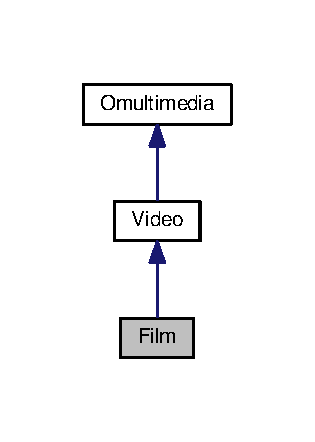
\includegraphics[width=151pt]{class_film__inherit__graph}
\end{center}
\end{figure}


Collaboration diagram for Film\+:
\nopagebreak
\begin{figure}[H]
\begin{center}
\leavevmode
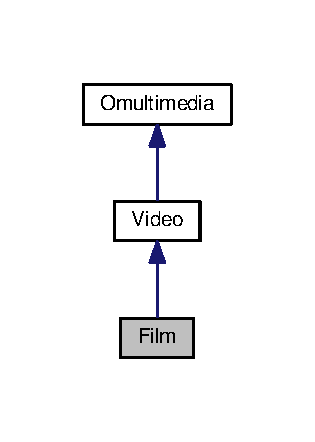
\includegraphics[width=151pt]{class_film__coll__graph}
\end{center}
\end{figure}
\subsection*{Public Member Functions}
\begin{DoxyCompactItemize}
\item 
\hypertarget{class_film_add96a21aaa3ae32a9bb860ddafeb48ff}{{\bfseries Film} (int num\+Chapitre, string nom\+Film, string path\+Film)}\label{class_film_add96a21aaa3ae32a9bb860ddafeb48ff}

\item 
\hypertarget{class_film_aee1f05dbc38270e72186bedfc55c7d74}{{\bfseries Film} (int $\ast$vet, int N, string nom\+Film, string path\+Film)}\label{class_film_aee1f05dbc38270e72186bedfc55c7d74}

\item 
\hypertarget{class_film_acc6f65afe85fdc48ff52072149664d22}{virtual int {\bfseries get\+Nombre\+Chapitre} () const }\label{class_film_acc6f65afe85fdc48ff52072149664d22}

\item 
\hypertarget{class_film_aeb014e6e9401a70e7787053a6e8bc6a1}{virtual int $\ast$ {\bfseries get\+Tableau\+Duree} () const }\label{class_film_aeb014e6e9401a70e7787053a6e8bc6a1}

\item 
\hypertarget{class_film_ac610b7fc13d8903e6c06af1864f2bcea}{virtual void {\bfseries set\+Nombre\+Chapitre} (int num\+Chapitre)}\label{class_film_ac610b7fc13d8903e6c06af1864f2bcea}

\item 
\hypertarget{class_film_a07054ea86fee34dbc716269dee9803cf}{virtual void {\bfseries set\+Tableau\+Duree} (const int $\ast$vet, int N)}\label{class_film_a07054ea86fee34dbc716269dee9803cf}

\item 
\hypertarget{class_film_a250b49e275035c8bcaec3cf1d0627b4e}{virtual void {\bfseries afficher\+Duree\+Chapitre} (ostream \&s) const }\label{class_film_a250b49e275035c8bcaec3cf1d0627b4e}

\item 
\hypertarget{class_film_aab7e0aacfdf61b43e3fecda2aad8d7c7}{virtual void {\bfseries liberer\+Memoire} ()}\label{class_film_aab7e0aacfdf61b43e3fecda2aad8d7c7}

\end{DoxyCompactItemize}


\subsection{Detailed Description}
The \hyperlink{class_film}{Film} class sous classe de \hyperlink{class_video}{Video}. 

The documentation for this class was generated from the following files\+:\begin{DoxyCompactItemize}
\item 
/cal/homes/fouotsap/\+Desktop/\+Fouotsap\+\_\+\+Foukmeniok\+\_\+\+Alain/cpp/Film.\+h\item 
/cal/homes/fouotsap/\+Desktop/\+Fouotsap\+\_\+\+Foukmeniok\+\_\+\+Alain/cpp/Film.\+cpp\end{DoxyCompactItemize}

\hypertarget{class_groupe}{\section{Groupe Class Reference}
\label{class_groupe}\index{Groupe@{Groupe}}
}


Inherits list$<$ Omultimedia\+Ptr $>$.

\subsection*{Public Member Functions}
\begin{DoxyCompactItemize}
\item 
\hypertarget{class_groupe_a69bd7f1c9400e287c531c9b5f1da19cb}{{\bfseries Groupe} (string group\+Name)}\label{class_groupe_a69bd7f1c9400e287c531c9b5f1da19cb}

\item 
\hypertarget{class_groupe_a37f0f8e74f1826265933503de8a45583}{virtual string {\bfseries get\+Group\+Name} () const }\label{class_groupe_a37f0f8e74f1826265933503de8a45583}

\item 
\hypertarget{class_groupe_ab4d1294beccf02aba10b704ef9c296b9}{virtual void {\bfseries afficher\+Attribut\+List} (ostream \&s) const }\label{class_groupe_ab4d1294beccf02aba10b704ef9c296b9}

\end{DoxyCompactItemize}


The documentation for this class was generated from the following files\+:\begin{DoxyCompactItemize}
\item 
/cal/homes/fouotsap/inf224/Groupe.\+h\item 
/cal/homes/fouotsap/inf224/Groupe.\+cpp\end{DoxyCompactItemize}

\hypertarget{structcppu_1_1_input_buffer}{\section{cppu\+:\+:Input\+Buffer Struct Reference}
\label{structcppu_1_1_input_buffer}\index{cppu\+::\+Input\+Buffer@{cppu\+::\+Input\+Buffer}}
}
\subsection*{Public Member Functions}
\begin{DoxyCompactItemize}
\item 
\hypertarget{structcppu_1_1_input_buffer_ac50e17e3cfb76a2983e5e3d4558b8144}{{\bfseries Input\+Buffer} (size\+\_\+t size)}\label{structcppu_1_1_input_buffer_ac50e17e3cfb76a2983e5e3d4558b8144}

\end{DoxyCompactItemize}
\subsection*{Public Attributes}
\begin{DoxyCompactItemize}
\item 
\hypertarget{structcppu_1_1_input_buffer_a85138068e2e10731e46784b1552bc354}{char $\ast$ {\bfseries buffer}}\label{structcppu_1_1_input_buffer_a85138068e2e10731e46784b1552bc354}

\item 
\hypertarget{structcppu_1_1_input_buffer_adbd6fb30fe51a192c9bbba6333016f31}{char $\ast$ {\bfseries begin}}\label{structcppu_1_1_input_buffer_adbd6fb30fe51a192c9bbba6333016f31}

\item 
\hypertarget{structcppu_1_1_input_buffer_ac9fb4f51a6db191e71976fcda20237c0}{char $\ast$ {\bfseries end}}\label{structcppu_1_1_input_buffer_ac9fb4f51a6db191e71976fcda20237c0}

\item 
\hypertarget{structcppu_1_1_input_buffer_a646b547733665524fa8b5de6b093ab11}{ssize\+\_\+t {\bfseries remaining}}\label{structcppu_1_1_input_buffer_a646b547733665524fa8b5de6b093ab11}

\end{DoxyCompactItemize}


The documentation for this struct was generated from the following file\+:\begin{DoxyCompactItemize}
\item 
/cal/homes/fouotsap/\+Desktop/\+Fouotsap\+\_\+\+Foukmeniok\+\_\+\+Alain/cpp/cppsocket.\+cpp\end{DoxyCompactItemize}

\hypertarget{class_omultimedia}{\section{Omultimedia Class Reference}
\label{class_omultimedia}\index{Omultimedia@{Omultimedia}}
}


Inherited by \hyperlink{class_photo}{Photo}, and \hyperlink{class_video}{Video}.

\subsection*{Public Member Functions}
\begin{DoxyCompactItemize}
\item 
\hypertarget{class_omultimedia_a7f1e73b963ad35cf904c1ca05836c90d}{{\bfseries Omultimedia} (string object\+\_\+name, string object\+\_\+pathname)}\label{class_omultimedia_a7f1e73b963ad35cf904c1ca05836c90d}

\item 
\hypertarget{class_omultimedia_a9f9f433c1156c1febf54b88037de8ddb}{virtual void {\bfseries set\+Object\+Name} (string object\+\_\+name)}\label{class_omultimedia_a9f9f433c1156c1febf54b88037de8ddb}

\item 
\hypertarget{class_omultimedia_a4e8aebf79dbc7759e9566eaa18f00b38}{virtual void {\bfseries set\+Object\+Pathname} (string object\+\_\+pathname)}\label{class_omultimedia_a4e8aebf79dbc7759e9566eaa18f00b38}

\item 
\hypertarget{class_omultimedia_ae6404617513dd4b667fee79b72be6fb0}{virtual string {\bfseries get\+Object\+Name} () const }\label{class_omultimedia_ae6404617513dd4b667fee79b72be6fb0}

\item 
\hypertarget{class_omultimedia_a6f503402124f2c086c62ca473b3295e4}{virtual string {\bfseries get\+Object\+Pathname} () const }\label{class_omultimedia_a6f503402124f2c086c62ca473b3295e4}

\item 
virtual void \hyperlink{class_omultimedia_ae8942bb1db61d92962a71bbe7512c037}{afficher\+Objet} (ostream \&s) const =0
\begin{DoxyCompactList}\small\item\em \hyperlink{class_omultimedia_ae8942bb1db61d92962a71bbe7512c037}{Omultimedia\+::afficher\+Objet}. \end{DoxyCompactList}\item 
\hypertarget{class_omultimedia_ab3836cd1744e98bdc6752ebd0283911e}{virtual void {\bfseries jouer\+Objet} (string nom\+Objet, string path) const =0}\label{class_omultimedia_ab3836cd1744e98bdc6752ebd0283911e}

\end{DoxyCompactItemize}


\subsection{Member Function Documentation}
\hypertarget{class_omultimedia_ae8942bb1db61d92962a71bbe7512c037}{\index{Omultimedia@{Omultimedia}!afficher\+Objet@{afficher\+Objet}}
\index{afficher\+Objet@{afficher\+Objet}!Omultimedia@{Omultimedia}}
\subsubsection[{afficher\+Objet}]{\setlength{\rightskip}{0pt plus 5cm}void Omultimedia\+::afficher\+Objet (
\begin{DoxyParamCaption}
\item[{ostream \&}]{s}
\end{DoxyParamCaption}
) const\hspace{0.3cm}{\ttfamily [pure virtual]}}}\label{class_omultimedia_ae8942bb1db61d92962a71bbe7512c037}


\hyperlink{class_omultimedia_ae8942bb1db61d92962a71bbe7512c037}{Omultimedia\+::afficher\+Objet}. 


\begin{DoxyParams}{Parameters}
{\em s} & flux de sortie(file,console,buffer de texte) \\
\hline
\end{DoxyParams}


Implemented in \hyperlink{class_photo_a6c80c6f056b2ec84cc30ad0afecd9806}{Photo}, and \hyperlink{class_video_a3a4dd11a3021cf824d98006498d0b2af}{Video}.



The documentation for this class was generated from the following files\+:\begin{DoxyCompactItemize}
\item 
/cal/homes/fouotsap/inf224/Omultimedia.\+h\item 
/cal/homes/fouotsap/inf224/Omultimedia.\+cpp\end{DoxyCompactItemize}

\hypertarget{class_photo}{\section{Photo Class Reference}
\label{class_photo}\index{Photo@{Photo}}
}


The \hyperlink{class_photo}{Photo} class sous classe d'objet multimedia.  




{\ttfamily \#include $<$Photo.\+h$>$}



Inheritance diagram for Photo\+:
\nopagebreak
\begin{figure}[H]
\begin{center}
\leavevmode
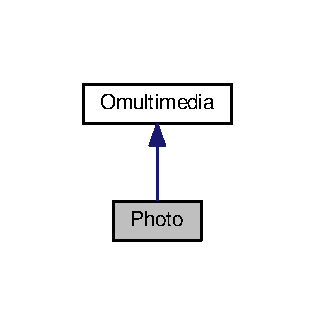
\includegraphics[width=151pt]{class_photo__inherit__graph}
\end{center}
\end{figure}


Collaboration diagram for Photo\+:
\nopagebreak
\begin{figure}[H]
\begin{center}
\leavevmode
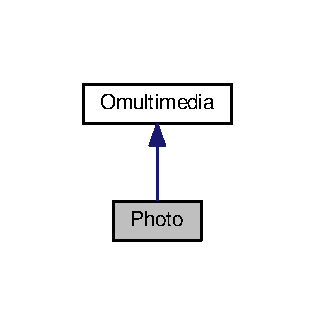
\includegraphics[width=151pt]{class_photo__coll__graph}
\end{center}
\end{figure}
\subsection*{Public Member Functions}
\begin{DoxyCompactItemize}
\item 
\hypertarget{class_photo_a4b68b4e4c551bbad82073932a0d3e800}{{\bfseries Photo} (unsigned int latitude, unsigned int longitude, string nom\+Photo, string path\+Photo)}\label{class_photo_a4b68b4e4c551bbad82073932a0d3e800}

\item 
\hypertarget{class_photo_a5d7841d5429264d5023baf921efd00b0}{unsigned int {\bfseries get\+Latitude\+Photo} () const }\label{class_photo_a5d7841d5429264d5023baf921efd00b0}

\item 
\hypertarget{class_photo_a081941cde635fe42bd017ef48b5f5ae6}{unsigned int {\bfseries get\+Longitude\+Photo} () const }\label{class_photo_a081941cde635fe42bd017ef48b5f5ae6}

\item 
\hypertarget{class_photo_aae3805bb2c61cb96cc11e7f09fe5bc1c}{void {\bfseries set\+Latitude\+Photo} (unsigned int latitude)}\label{class_photo_aae3805bb2c61cb96cc11e7f09fe5bc1c}

\item 
\hypertarget{class_photo_ab58d0b90b56098457653ffeddb1e03ff}{void {\bfseries set\+Longitude\+Photo} (unsigned int longitude)}\label{class_photo_ab58d0b90b56098457653ffeddb1e03ff}

\item 
void \hyperlink{class_photo_a6c80c6f056b2ec84cc30ad0afecd9806}{afficher\+Objet} (ostream \&s) const override
\begin{DoxyCompactList}\small\item\em \hyperlink{class_omultimedia_ae8942bb1db61d92962a71bbe7512c037}{Omultimedia\+::afficher\+Objet}. \end{DoxyCompactList}\item 
void \hyperlink{class_photo_a5b9e3f3f830c4fd02f930fee9dc8dfb2}{jouer\+Objet} (string nom\+Objet, string path) const override
\begin{DoxyCompactList}\small\item\em jouer\+Objet joue un objet multimedia à partir de son nom et son path \end{DoxyCompactList}\end{DoxyCompactItemize}


\subsection{Detailed Description}
The \hyperlink{class_photo}{Photo} class sous classe d'objet multimedia. 

\subsection{Member Function Documentation}
\hypertarget{class_photo_a6c80c6f056b2ec84cc30ad0afecd9806}{\index{Photo@{Photo}!afficher\+Objet@{afficher\+Objet}}
\index{afficher\+Objet@{afficher\+Objet}!Photo@{Photo}}
\subsubsection[{afficher\+Objet}]{\setlength{\rightskip}{0pt plus 5cm}void Photo\+::afficher\+Objet (
\begin{DoxyParamCaption}
\item[{ostream \&}]{s}
\end{DoxyParamCaption}
) const\hspace{0.3cm}{\ttfamily [override]}, {\ttfamily [virtual]}}}\label{class_photo_a6c80c6f056b2ec84cc30ad0afecd9806}


\hyperlink{class_omultimedia_ae8942bb1db61d92962a71bbe7512c037}{Omultimedia\+::afficher\+Objet}. 


\begin{DoxyParams}{Parameters}
{\em s} & flux de sortie(file,console,buffer de texte) \\
\hline
\end{DoxyParams}


Implements \hyperlink{class_omultimedia_ae8942bb1db61d92962a71bbe7512c037}{Omultimedia}.

\hypertarget{class_photo_a5b9e3f3f830c4fd02f930fee9dc8dfb2}{\index{Photo@{Photo}!jouer\+Objet@{jouer\+Objet}}
\index{jouer\+Objet@{jouer\+Objet}!Photo@{Photo}}
\subsubsection[{jouer\+Objet}]{\setlength{\rightskip}{0pt plus 5cm}void Photo\+::jouer\+Objet (
\begin{DoxyParamCaption}
\item[{string}]{nom\+Objet, }
\item[{string}]{path}
\end{DoxyParamCaption}
) const\hspace{0.3cm}{\ttfamily [override]}, {\ttfamily [virtual]}}}\label{class_photo_a5b9e3f3f830c4fd02f930fee9dc8dfb2}


jouer\+Objet joue un objet multimedia à partir de son nom et son path 


\begin{DoxyParams}{Parameters}
{\em nom\+Objet} & \\
\hline
{\em path} & c'est une méthode abstraite qui sera redéfinie dans chacune des sous classes \\
\hline
\end{DoxyParams}


Implements \hyperlink{class_omultimedia_ab3836cd1744e98bdc6752ebd0283911e}{Omultimedia}.



The documentation for this class was generated from the following files\+:\begin{DoxyCompactItemize}
\item 
/cal/homes/fouotsap/\+Desktop/\+Fouotsap\+\_\+\+Foukmeniok\+\_\+\+Alain/cpp/Photo.\+h\item 
/cal/homes/fouotsap/\+Desktop/\+Fouotsap\+\_\+\+Foukmeniok\+\_\+\+Alain/cpp/Photo.\+cpp\end{DoxyCompactItemize}

\hypertarget{classcppu_1_1_server_socket}{\section{cppu\+:\+:Server\+Socket Class Reference}
\label{classcppu_1_1_server_socket}\index{cppu\+::\+Server\+Socket@{cppu\+::\+Server\+Socket}}
}


T\+C\+P/\+I\+P server socket. This class implements a T\+C\+P/\+I\+P socket that waits for requests to come in over the network. A\+F\+\_\+\+I\+N\+E\+T connections following the I\+Pv4 Internet protocol are supported.  




{\ttfamily \#include $<$cppsocket.\+h$>$}

\subsection*{Public Member Functions}
\begin{DoxyCompactItemize}
\item 
\hypertarget{classcppu_1_1_server_socket_a57138f5a7d2e8af35228c8985385c494}{\hyperlink{classcppu_1_1_server_socket_a57138f5a7d2e8af35228c8985385c494}{Server\+Socket} ()}\label{classcppu_1_1_server_socket_a57138f5a7d2e8af35228c8985385c494}

\begin{DoxyCompactList}\small\item\em Creates a new server socket. Creates a listening socket that waits for connection requests by T\+C\+P/\+I\+P clients. \end{DoxyCompactList}\item 
virtual \hyperlink{classcppu_1_1_socket}{Socket} $\ast$ \hyperlink{classcppu_1_1_server_socket_af08ebcb886fc778d195fb622f7b96b8b}{accept} ()
\begin{DoxyCompactList}\small\item\em Accepts a new connection request and returns the corresponding socket. By default, this function blocks the caller until a connection is present. \end{DoxyCompactList}\item 
virtual int \hyperlink{classcppu_1_1_server_socket_a255dfdccba51c7cdbcb6733c6c3f6ffa}{bind} (int port, int backlog=50)
\begin{DoxyCompactList}\small\item\em Assigns the socket to the local address. The socket must be bound before using it. \end{DoxyCompactList}\item 
\hypertarget{classcppu_1_1_server_socket_ae7647cfb5beaf504a846f6ecfdd197c4}{virtual int \hyperlink{classcppu_1_1_server_socket_ae7647cfb5beaf504a846f6ecfdd197c4}{close} ()}\label{classcppu_1_1_server_socket_ae7647cfb5beaf504a846f6ecfdd197c4}

\begin{DoxyCompactList}\small\item\em Closes the socket. \end{DoxyCompactList}\item 
\hypertarget{classcppu_1_1_server_socket_aa3ca8fed354955eeb45af3a2021c04cb}{bool \hyperlink{classcppu_1_1_server_socket_aa3ca8fed354955eeb45af3a2021c04cb}{is\+Closed} () const }\label{classcppu_1_1_server_socket_aa3ca8fed354955eeb45af3a2021c04cb}

\begin{DoxyCompactList}\small\item\em Returns true if the socket has been closed. \end{DoxyCompactList}\item 
\hypertarget{classcppu_1_1_server_socket_a905d85f63fdca46ed5ee44eb00e211d1}{int \hyperlink{classcppu_1_1_server_socket_a905d85f63fdca46ed5ee44eb00e211d1}{descriptor} ()}\label{classcppu_1_1_server_socket_a905d85f63fdca46ed5ee44eb00e211d1}

\begin{DoxyCompactList}\small\item\em Returns the Unix descriptor of the socket. \end{DoxyCompactList}\item 
\hypertarget{classcppu_1_1_server_socket_a0fbd0ee42bcfecf2e749279c4b94b0b3}{int \hyperlink{classcppu_1_1_server_socket_a0fbd0ee42bcfecf2e749279c4b94b0b3}{set\+Receive\+Buffer\+Size} (int size)}\label{classcppu_1_1_server_socket_a0fbd0ee42bcfecf2e749279c4b94b0b3}

\begin{DoxyCompactList}\small\item\em Sets the S\+O\+\_\+\+R\+C\+V\+B\+U\+F option to the specified value. \end{DoxyCompactList}\item 
\hypertarget{classcppu_1_1_server_socket_a09d0494cc0f65abe496b9c940d2920ed}{int \hyperlink{classcppu_1_1_server_socket_a09d0494cc0f65abe496b9c940d2920ed}{set\+Reuse\+Address} (bool)}\label{classcppu_1_1_server_socket_a09d0494cc0f65abe496b9c940d2920ed}

\begin{DoxyCompactList}\small\item\em Enables/disables the S\+O\+\_\+\+R\+E\+U\+S\+E\+A\+D\+D\+R socket option. \end{DoxyCompactList}\item 
\hypertarget{classcppu_1_1_server_socket_a0ceb984eab0cdd9c7c8e62658a521175}{int \hyperlink{classcppu_1_1_server_socket_a0ceb984eab0cdd9c7c8e62658a521175}{set\+So\+Timeout} (int timeout)}\label{classcppu_1_1_server_socket_a0ceb984eab0cdd9c7c8e62658a521175}

\begin{DoxyCompactList}\small\item\em Enables/disables S\+O\+\_\+\+T\+I\+M\+E\+O\+U\+T with the specified timeout (in milliseconds). \end{DoxyCompactList}\item 
\hypertarget{classcppu_1_1_server_socket_ac5f6da333208cce9ca4d5392259a0a6b}{int \hyperlink{classcppu_1_1_server_socket_ac5f6da333208cce9ca4d5392259a0a6b}{set\+Tcp\+No\+Delay} (bool)}\label{classcppu_1_1_server_socket_ac5f6da333208cce9ca4d5392259a0a6b}

\begin{DoxyCompactList}\small\item\em Turns on/off T\+C\+P coalescence (useful in some cases to avoid delays). \end{DoxyCompactList}\end{DoxyCompactItemize}
\subsection*{Protected Member Functions}
\begin{DoxyCompactItemize}
\item 
\hypertarget{classcppu_1_1_server_socket_a23d038275576d0a969072eb334f7b84f}{virtual \hyperlink{classcppu_1_1_socket}{Socket} $\ast$ {\bfseries create\+Socket} (int sockfd)}\label{classcppu_1_1_server_socket_a23d038275576d0a969072eb334f7b84f}

\end{DoxyCompactItemize}


\subsection{Detailed Description}
T\+C\+P/\+I\+P server socket. This class implements a T\+C\+P/\+I\+P socket that waits for requests to come in over the network. A\+F\+\_\+\+I\+N\+E\+T connections following the I\+Pv4 Internet protocol are supported. 

\begin{DoxyNote}{Note}
T\+C\+P/\+I\+P sockets do not preserve record boundaries, 
\end{DoxyNote}
\begin{DoxySeeAlso}{See also}
\hyperlink{classcppu_1_1_socket_buffer}{Socket\+Buffer} for a solution. 
\end{DoxySeeAlso}


\subsection{Member Function Documentation}
\hypertarget{classcppu_1_1_server_socket_af08ebcb886fc778d195fb622f7b96b8b}{\index{cppu\+::\+Server\+Socket@{cppu\+::\+Server\+Socket}!accept@{accept}}
\index{accept@{accept}!cppu\+::\+Server\+Socket@{cppu\+::\+Server\+Socket}}
\subsubsection[{accept}]{\setlength{\rightskip}{0pt plus 5cm}{\bf Socket} $\ast$ cppu\+::\+Server\+Socket\+::accept (
\begin{DoxyParamCaption}
{}
\end{DoxyParamCaption}
)\hspace{0.3cm}{\ttfamily [virtual]}}}\label{classcppu_1_1_server_socket_af08ebcb886fc778d195fb622f7b96b8b}


Accepts a new connection request and returns the corresponding socket. By default, this function blocks the caller until a connection is present. 

\begin{DoxyReturn}{Returns}
the new \hyperlink{classcppu_1_1_socket}{Socket} or nullptr on error. 
\end{DoxyReturn}
\hypertarget{classcppu_1_1_server_socket_a255dfdccba51c7cdbcb6733c6c3f6ffa}{\index{cppu\+::\+Server\+Socket@{cppu\+::\+Server\+Socket}!bind@{bind}}
\index{bind@{bind}!cppu\+::\+Server\+Socket@{cppu\+::\+Server\+Socket}}
\subsubsection[{bind}]{\setlength{\rightskip}{0pt plus 5cm}int cppu\+::\+Server\+Socket\+::bind (
\begin{DoxyParamCaption}
\item[{int}]{port, }
\item[{int}]{backlog = {\ttfamily 50}}
\end{DoxyParamCaption}
)\hspace{0.3cm}{\ttfamily [virtual]}}}\label{classcppu_1_1_server_socket_a255dfdccba51c7cdbcb6733c6c3f6ffa}


Assigns the socket to the local address. The socket must be bound before using it. 

\begin{DoxyReturn}{Returns}
0 on success or a negative value on error which is one of \hyperlink{classcppu_1_1_socket_a49ea5cb079bd7ae97ecf7eb30c9d9e5f}{Socket\+::\+Errors} 
\end{DoxyReturn}


The documentation for this class was generated from the following files\+:\begin{DoxyCompactItemize}
\item 
/cal/homes/fouotsap/inf224/cppsocket.\+h\item 
/cal/homes/fouotsap/inf224/cppsocket.\+cpp\end{DoxyCompactItemize}

\hypertarget{classcppu_1_1_socket}{\section{cppu\+:\+:Socket Class Reference}
\label{classcppu_1_1_socket}\index{cppu\+::\+Socket@{cppu\+::\+Socket}}
}


T\+C\+P/\+I\+P or U\+D\+P/\+Datagram socket. This class encapsulates a T\+C\+P/\+I\+P or U\+D\+P/\+Datagram socket. A\+F\+\_\+\+I\+N\+E\+T connections following the I\+Pv4 Internet protocol are supported.  




{\ttfamily \#include $<$cppsocket.\+h$>$}

\subsection*{Public Types}
\begin{DoxyCompactItemize}
\item 
enum \hyperlink{classcppu_1_1_socket_a49ea5cb079bd7ae97ecf7eb30c9d9e5f}{Errors} \{ {\bfseries Failed} = -\/1, 
{\bfseries Invalid\+Socket} = -\/2, 
{\bfseries Unknown\+Host} = -\/3
 \}
\begin{DoxyCompactList}\small\item\em \hyperlink{classcppu_1_1_socket}{Socket} errors. \end{DoxyCompactList}\end{DoxyCompactItemize}
\subsection*{Public Member Functions}
\begin{DoxyCompactItemize}
\item 
\hyperlink{classcppu_1_1_socket_ae73b9b629fe443f650203d938f61a279}{Socket} (int type=S\+O\+C\+K\+\_\+\+S\+T\+R\+E\+A\+M)
\begin{DoxyCompactList}\small\item\em Creates a new \hyperlink{classcppu_1_1_socket}{Socket}. Creates a A\+F\+\_\+\+I\+N\+E\+T socket using the I\+Pv4 Internet protocol. Type can be\+: \end{DoxyCompactList}\item 
\hypertarget{classcppu_1_1_socket_a8404e4e80cc625a4be32aacc879bb237}{\hyperlink{classcppu_1_1_socket_a8404e4e80cc625a4be32aacc879bb237}{Socket} (int type, int sockfd)}\label{classcppu_1_1_socket_a8404e4e80cc625a4be32aacc879bb237}

\begin{DoxyCompactList}\small\item\em Creates a \hyperlink{classcppu_1_1_socket}{Socket} object from an existing socket file descriptor. \end{DoxyCompactList}\item 
\hypertarget{classcppu_1_1_socket_ae26733a0b7d8a5fb5544d2d069152de7}{virtual \hyperlink{classcppu_1_1_socket_ae26733a0b7d8a5fb5544d2d069152de7}{$\sim$\+Socket} ()}\label{classcppu_1_1_socket_ae26733a0b7d8a5fb5544d2d069152de7}

\begin{DoxyCompactList}\small\item\em Destructor (closes the socket). \end{DoxyCompactList}\item 
virtual int \hyperlink{classcppu_1_1_socket_a7b876dcaff0babaffde41575f9b19d64}{bind} (int port)
\begin{DoxyCompactList}\small\item\em Assigns the socket to the local address. Typically used for U\+D\+P/\+Datagram sockets,. \end{DoxyCompactList}\item 
virtual int \hyperlink{classcppu_1_1_socket_a5698a3a7c6c203676c6de5e5559a0a7f}{bind} (const std\+::string \&host, int port)
\begin{DoxyCompactList}\small\item\em Assigns the socket to an address. Typically used for U\+D\+P/\+Datagram sockets,. \end{DoxyCompactList}\item 
virtual int \hyperlink{classcppu_1_1_socket_af6db3840caee709738f0e2a9ff814e5d}{connect} (const std\+::string \&host, int port)
\begin{DoxyCompactList}\small\item\em Connects the socket to an address. Typically used for T\+C\+P/\+I\+P sockets on the client side,. \end{DoxyCompactList}\item 
virtual int \hyperlink{classcppu_1_1_socket_ab958ef8a0f0495cf3a1c57a2ad4a34fc}{close} ()
\begin{DoxyCompactList}\small\item\em Closes the socket. \end{DoxyCompactList}\item 
\hypertarget{classcppu_1_1_socket_a726c2e6be413fe4e0584a23a173ae540}{bool \hyperlink{classcppu_1_1_socket_a726c2e6be413fe4e0584a23a173ae540}{is\+Closed} () const }\label{classcppu_1_1_socket_a726c2e6be413fe4e0584a23a173ae540}

\begin{DoxyCompactList}\small\item\em Returns true if the socket has been closed. \end{DoxyCompactList}\item 
\hypertarget{classcppu_1_1_socket_a06a8fcd9518e6a3e8b33bb64f7fb9036}{int \hyperlink{classcppu_1_1_socket_a06a8fcd9518e6a3e8b33bb64f7fb9036}{descriptor} ()}\label{classcppu_1_1_socket_a06a8fcd9518e6a3e8b33bb64f7fb9036}

\begin{DoxyCompactList}\small\item\em Returns the Unix descriptor of the socket. \end{DoxyCompactList}\item 
ssize\+\_\+t \hyperlink{classcppu_1_1_socket_aeac77f859159715e2d63a5a0dc118788}{send} (const void $\ast$buf, size\+\_\+t len, int flags=0)
\begin{DoxyCompactList}\small\item\em Sends data to a connected socket. Sends {\itshape len} bytes to a T\+C\+P/\+I\+P socket using the Unix \hyperlink{classcppu_1_1_socket_aeac77f859159715e2d63a5a0dc118788}{send()} function (. \end{DoxyCompactList}\item 
ssize\+\_\+t \hyperlink{classcppu_1_1_socket_a37c382af52cc02f92c0e19a0c6e0e04f}{receive} (void $\ast$buf, size\+\_\+t len, int flags=0)
\begin{DoxyCompactList}\small\item\em Receives data from a connected socket. Reads at most {\itshape len} bytes from a T\+C\+P/\+I\+P socket using the Unix recv() function. By default, this function blocks the caller until data is present (. \end{DoxyCompactList}\item 
ssize\+\_\+t \hyperlink{classcppu_1_1_socket_a31ff5137959aa4e52d4bcdd53e0b0069}{send\+To} (const void $\ast$buf, size\+\_\+t len, int flags, const struct sockaddr $\ast$dest\+\_\+addr, socklen\+\_\+t addrlen)
\begin{DoxyCompactList}\small\item\em Sends data to a datagram socket. Sends {\itshape len} bytes to a datagram socket using the Unix sendto() function. \end{DoxyCompactList}\item 
ssize\+\_\+t \hyperlink{classcppu_1_1_socket_abd460be82deeb29e730fc83f871e51c4}{receive\+From} (void $\ast$buf, size\+\_\+t len, int flags, struct sockaddr $\ast$src\+\_\+addr, socklen\+\_\+t $\ast$addrlen)
\begin{DoxyCompactList}\small\item\em Receives data from datagram socket. Reads at most {\itshape len} bytes from a datagram socket using the Unix recvfrom() function. By default, this function blocks the caller until data is present (. \end{DoxyCompactList}\item 
\hypertarget{classcppu_1_1_socket_a06c6838f267e5a0ba74558da946efb90}{virtual void \hyperlink{classcppu_1_1_socket_a06c6838f267e5a0ba74558da946efb90}{shutdown\+Input} ()}\label{classcppu_1_1_socket_a06c6838f267e5a0ba74558da946efb90}

\begin{DoxyCompactList}\small\item\em Disables further receive operations. \end{DoxyCompactList}\item 
\hypertarget{classcppu_1_1_socket_a97ee9ef3bf9fdecd6ae6f2b583b34d0e}{virtual void \hyperlink{classcppu_1_1_socket_a97ee9ef3bf9fdecd6ae6f2b583b34d0e}{shutdown\+Output} ()}\label{classcppu_1_1_socket_a97ee9ef3bf9fdecd6ae6f2b583b34d0e}

\begin{DoxyCompactList}\small\item\em Disables further send operations. \end{DoxyCompactList}\item 
\hypertarget{classcppu_1_1_socket_af172d5c78f63713988b0a6bf66851be7}{int \hyperlink{classcppu_1_1_socket_af172d5c78f63713988b0a6bf66851be7}{set\+Receive\+Buffer\+Size} (int size)}\label{classcppu_1_1_socket_af172d5c78f63713988b0a6bf66851be7}

\begin{DoxyCompactList}\small\item\em Sets the size of the T\+C\+P/\+I\+P input buffer. \end{DoxyCompactList}\item 
\hypertarget{classcppu_1_1_socket_a27b7fe34e172ad1f97c304d2786f624a}{int \hyperlink{classcppu_1_1_socket_a27b7fe34e172ad1f97c304d2786f624a}{set\+Reuse\+Address} (bool)}\label{classcppu_1_1_socket_a27b7fe34e172ad1f97c304d2786f624a}

\begin{DoxyCompactList}\small\item\em Enables/disables the S\+O\+\_\+\+R\+E\+U\+S\+E\+A\+D\+D\+R socket option. \end{DoxyCompactList}\item 
\hypertarget{classcppu_1_1_socket_aefda954454d860fa6a6d41b3d5cd26db}{int \hyperlink{classcppu_1_1_socket_aefda954454d860fa6a6d41b3d5cd26db}{set\+Send\+Buffer\+Size} (int size)}\label{classcppu_1_1_socket_aefda954454d860fa6a6d41b3d5cd26db}

\begin{DoxyCompactList}\small\item\em Sets the size of the T\+C\+P/\+I\+P output buffer. \end{DoxyCompactList}\item 
\hypertarget{classcppu_1_1_socket_ae87eb0335c072f765bf2b6a47162e7f5}{int \hyperlink{classcppu_1_1_socket_ae87eb0335c072f765bf2b6a47162e7f5}{set\+So\+Linger} (bool, int linger)}\label{classcppu_1_1_socket_ae87eb0335c072f765bf2b6a47162e7f5}

\begin{DoxyCompactList}\small\item\em Enables/disables S\+O\+\_\+\+L\+I\+N\+G\+E\+R with the specified linger time in seconds. \end{DoxyCompactList}\item 
\hypertarget{classcppu_1_1_socket_ae5dea30a1cae2dbdbdaf11a9f7ffa444}{int \hyperlink{classcppu_1_1_socket_ae5dea30a1cae2dbdbdaf11a9f7ffa444}{set\+So\+Timeout} (int timeout)}\label{classcppu_1_1_socket_ae5dea30a1cae2dbdbdaf11a9f7ffa444}

\begin{DoxyCompactList}\small\item\em Enables/disables S\+O\+\_\+\+T\+I\+M\+E\+O\+U\+T with the specified timeout (in milliseconds). \end{DoxyCompactList}\item 
\hypertarget{classcppu_1_1_socket_a6b29a9e12926b07f65b8dc52176131c5}{int \hyperlink{classcppu_1_1_socket_a6b29a9e12926b07f65b8dc52176131c5}{set\+Tcp\+No\+Delay} (bool)}\label{classcppu_1_1_socket_a6b29a9e12926b07f65b8dc52176131c5}

\begin{DoxyCompactList}\small\item\em Enables/disables T\+C\+P\+\_\+\+N\+O\+D\+E\+L\+A\+Y (turns on/off T\+C\+P coalescence). \end{DoxyCompactList}\item 
\hypertarget{classcppu_1_1_socket_a677726fbe23c7b4117c648d54fd217a4}{int \hyperlink{classcppu_1_1_socket_a677726fbe23c7b4117c648d54fd217a4}{get\+Receive\+Buffer\+Size} () const }\label{classcppu_1_1_socket_a677726fbe23c7b4117c648d54fd217a4}

\begin{DoxyCompactList}\small\item\em Gets the size of the T\+C\+P/\+I\+P input buffer. \end{DoxyCompactList}\item 
\hypertarget{classcppu_1_1_socket_a8b16f99014bf2050394f34b4f0963e8f}{bool \hyperlink{classcppu_1_1_socket_a8b16f99014bf2050394f34b4f0963e8f}{get\+Reuse\+Address} () const }\label{classcppu_1_1_socket_a8b16f99014bf2050394f34b4f0963e8f}

\begin{DoxyCompactList}\small\item\em Gets S\+O\+\_\+\+R\+E\+U\+S\+E\+A\+D\+D\+R state. \end{DoxyCompactList}\item 
\hypertarget{classcppu_1_1_socket_a98fe83074255461c25ac72fcfa974404}{int \hyperlink{classcppu_1_1_socket_a98fe83074255461c25ac72fcfa974404}{get\+Send\+Buffer\+Size} () const }\label{classcppu_1_1_socket_a98fe83074255461c25ac72fcfa974404}

\begin{DoxyCompactList}\small\item\em Gets the size of the T\+C\+P/\+I\+P output buffer. \end{DoxyCompactList}\item 
\hypertarget{classcppu_1_1_socket_a50c713d9a283096cc98767b432d5393b}{bool \hyperlink{classcppu_1_1_socket_a50c713d9a283096cc98767b432d5393b}{get\+So\+Linger} (int \&linger) const }\label{classcppu_1_1_socket_a50c713d9a283096cc98767b432d5393b}

\begin{DoxyCompactList}\small\item\em Gets S\+O\+\_\+\+L\+I\+N\+G\+E\+R state and the specified linger time in seconds. \end{DoxyCompactList}\item 
\hypertarget{classcppu_1_1_socket_a43a77728f6890f4e0473c6d949f7c9c4}{int \hyperlink{classcppu_1_1_socket_a43a77728f6890f4e0473c6d949f7c9c4}{get\+So\+Timeout} () const }\label{classcppu_1_1_socket_a43a77728f6890f4e0473c6d949f7c9c4}

\begin{DoxyCompactList}\small\item\em Gets S\+O\+\_\+\+T\+I\+M\+E\+O\+U\+T value. \end{DoxyCompactList}\item 
\hypertarget{classcppu_1_1_socket_aaa9812fdb949d4fbbb2546d9c8ebd3aa}{bool \hyperlink{classcppu_1_1_socket_aaa9812fdb949d4fbbb2546d9c8ebd3aa}{get\+Tcp\+No\+Delay} () const }\label{classcppu_1_1_socket_aaa9812fdb949d4fbbb2546d9c8ebd3aa}

\begin{DoxyCompactList}\small\item\em Gets T\+C\+P\+\_\+\+N\+O\+D\+E\+L\+A\+Y state. \end{DoxyCompactList}\item 
\hypertarget{classcppu_1_1_socket_a73d529332eae6048b321b381354e6bea}{virtual int \hyperlink{classcppu_1_1_socket_a73d529332eae6048b321b381354e6bea}{set\+Local\+Address} (struct sockaddr\+\_\+in \&addr, int port)}\label{classcppu_1_1_socket_a73d529332eae6048b321b381354e6bea}

\begin{DoxyCompactList}\small\item\em Initializes a local I\+N\+E\+T4 address, returns 0 on success, -\/1 otherwise. \end{DoxyCompactList}\item 
\hypertarget{classcppu_1_1_socket_aec26c9f6372f7ed2ec383fc98cbb6458}{virtual int \hyperlink{classcppu_1_1_socket_aec26c9f6372f7ed2ec383fc98cbb6458}{set\+Address} (struct sockaddr\+\_\+in \&addr, const std\+::string \&host, int port)}\label{classcppu_1_1_socket_aec26c9f6372f7ed2ec383fc98cbb6458}

\begin{DoxyCompactList}\small\item\em Initializes a remote I\+N\+E\+T4 address, returns 0 on success, -\/1 otherwise. \end{DoxyCompactList}\end{DoxyCompactItemize}
\subsection*{Friends}
\begin{DoxyCompactItemize}
\item 
\hypertarget{classcppu_1_1_socket_a11a8bb11feaafab939278a8285afa567}{class {\bfseries Server\+Socket}}\label{classcppu_1_1_socket_a11a8bb11feaafab939278a8285afa567}

\end{DoxyCompactItemize}


\subsection{Detailed Description}
T\+C\+P/\+I\+P or U\+D\+P/\+Datagram socket. This class encapsulates a T\+C\+P/\+I\+P or U\+D\+P/\+Datagram socket. A\+F\+\_\+\+I\+N\+E\+T connections following the I\+Pv4 Internet protocol are supported. 

\begin{DoxyNote}{Note}
\hyperlink{classcppu_1_1_server_socket}{Server\+Socket} should be used on the server side (
\end{DoxyNote}
\begin{DoxySeeAlso}{See also}
\hyperlink{classcppu_1_1_server_socket}{Server\+Socket}). 
\end{DoxySeeAlso}
\begin{DoxyNote}{Note}
S\+I\+G\+P\+I\+P\+E signals are ignored when using Linux, B\+S\+D or M\+A\+C\+O\+S\+X. 

T\+C\+P/\+I\+P sockets do not preserve record boundaries, 
\end{DoxyNote}
\begin{DoxySeeAlso}{See also}
\hyperlink{classcppu_1_1_socket_buffer}{Socket\+Buffer} for a solution. 
\end{DoxySeeAlso}


\subsection{Member Enumeration Documentation}
\hypertarget{classcppu_1_1_socket_a49ea5cb079bd7ae97ecf7eb30c9d9e5f}{\index{cppu\+::\+Socket@{cppu\+::\+Socket}!Errors@{Errors}}
\index{Errors@{Errors}!cppu\+::\+Socket@{cppu\+::\+Socket}}
\subsubsection[{Errors}]{\setlength{\rightskip}{0pt plus 5cm}enum {\bf cppu\+::\+Socket\+::\+Errors}}}\label{classcppu_1_1_socket_a49ea5cb079bd7ae97ecf7eb30c9d9e5f}


\hyperlink{classcppu_1_1_socket}{Socket} errors. 


\begin{DoxyItemize}
\item Socket\+::\+Failed (-\/1)\+: connection error (could not connect, could not bind, etc.)
\item Socket\+::\+Invalid\+Socket (-\/2)\+: invalid socket or wrong socket type
\item Socket\+::\+Unknown\+Host (-\/3)\+: could not reach host 
\end{DoxyItemize}

\subsection{Constructor \& Destructor Documentation}
\hypertarget{classcppu_1_1_socket_ae73b9b629fe443f650203d938f61a279}{\index{cppu\+::\+Socket@{cppu\+::\+Socket}!Socket@{Socket}}
\index{Socket@{Socket}!cppu\+::\+Socket@{cppu\+::\+Socket}}
\subsubsection[{Socket}]{\setlength{\rightskip}{0pt plus 5cm}cppu\+::\+Socket\+::\+Socket (
\begin{DoxyParamCaption}
\item[{int}]{type = {\ttfamily SOCK\+\_\+STREAM}}
\end{DoxyParamCaption}
)}}\label{classcppu_1_1_socket_ae73b9b629fe443f650203d938f61a279}


Creates a new \hyperlink{classcppu_1_1_socket}{Socket}. Creates a A\+F\+\_\+\+I\+N\+E\+T socket using the I\+Pv4 Internet protocol. Type can be\+: 


\begin{DoxyItemize}
\item S\+O\+C\+K\+\_\+\+S\+T\+R\+E\+A\+M (the default) for T\+C\+P/\+I\+P connected stream sockets
\item S\+O\+C\+K\+\_\+\+D\+G\+R\+A\+M for U\+D\+P/datagram sockets 
\end{DoxyItemize}

\subsection{Member Function Documentation}
\hypertarget{classcppu_1_1_socket_a7b876dcaff0babaffde41575f9b19d64}{\index{cppu\+::\+Socket@{cppu\+::\+Socket}!bind@{bind}}
\index{bind@{bind}!cppu\+::\+Socket@{cppu\+::\+Socket}}
\subsubsection[{bind}]{\setlength{\rightskip}{0pt plus 5cm}int cppu\+::\+Socket\+::bind (
\begin{DoxyParamCaption}
\item[{int}]{port}
\end{DoxyParamCaption}
)\hspace{0.3cm}{\ttfamily [virtual]}}}\label{classcppu_1_1_socket_a7b876dcaff0babaffde41575f9b19d64}


Assigns the socket to the local address. Typically used for U\+D\+P/\+Datagram sockets,. 

\begin{DoxySeeAlso}{See also}
Unix \hyperlink{classcppu_1_1_socket_a7b876dcaff0babaffde41575f9b19d64}{bind()} system call for details. 
\end{DoxySeeAlso}
\begin{DoxyReturn}{Returns}
0 on success or a negative value on error which is one of \hyperlink{classcppu_1_1_socket_a49ea5cb079bd7ae97ecf7eb30c9d9e5f}{Socket\+::\+Errors} 
\end{DoxyReturn}
\hypertarget{classcppu_1_1_socket_a5698a3a7c6c203676c6de5e5559a0a7f}{\index{cppu\+::\+Socket@{cppu\+::\+Socket}!bind@{bind}}
\index{bind@{bind}!cppu\+::\+Socket@{cppu\+::\+Socket}}
\subsubsection[{bind}]{\setlength{\rightskip}{0pt plus 5cm}virtual int cppu\+::\+Socket\+::bind (
\begin{DoxyParamCaption}
\item[{const std\+::string \&}]{host, }
\item[{int}]{port}
\end{DoxyParamCaption}
)\hspace{0.3cm}{\ttfamily [virtual]}}}\label{classcppu_1_1_socket_a5698a3a7c6c203676c6de5e5559a0a7f}


Assigns the socket to an address. Typically used for U\+D\+P/\+Datagram sockets,. 

\begin{DoxySeeAlso}{See also}
Unix \hyperlink{classcppu_1_1_socket_a7b876dcaff0babaffde41575f9b19d64}{bind()} system call for details. 
\end{DoxySeeAlso}
\begin{DoxyReturn}{Returns}
0 on success or a negative value on error which is one of \hyperlink{classcppu_1_1_socket_a49ea5cb079bd7ae97ecf7eb30c9d9e5f}{Socket\+::\+Errors} 
\end{DoxyReturn}
\hypertarget{classcppu_1_1_socket_ab958ef8a0f0495cf3a1c57a2ad4a34fc}{\index{cppu\+::\+Socket@{cppu\+::\+Socket}!close@{close}}
\index{close@{close}!cppu\+::\+Socket@{cppu\+::\+Socket}}
\subsubsection[{close}]{\setlength{\rightskip}{0pt plus 5cm}int cppu\+::\+Socket\+::close (
\begin{DoxyParamCaption}
{}
\end{DoxyParamCaption}
)\hspace{0.3cm}{\ttfamily [virtual]}}}\label{classcppu_1_1_socket_ab958ef8a0f0495cf3a1c57a2ad4a34fc}


Closes the socket. 

\begin{DoxyReturn}{Returns}
0 on success and -\/1 on error. 
\end{DoxyReturn}
\hypertarget{classcppu_1_1_socket_af6db3840caee709738f0e2a9ff814e5d}{\index{cppu\+::\+Socket@{cppu\+::\+Socket}!connect@{connect}}
\index{connect@{connect}!cppu\+::\+Socket@{cppu\+::\+Socket}}
\subsubsection[{connect}]{\setlength{\rightskip}{0pt plus 5cm}int cppu\+::\+Socket\+::connect (
\begin{DoxyParamCaption}
\item[{const std\+::string \&}]{host, }
\item[{int}]{port}
\end{DoxyParamCaption}
)\hspace{0.3cm}{\ttfamily [virtual]}}}\label{classcppu_1_1_socket_af6db3840caee709738f0e2a9ff814e5d}


Connects the socket to an address. Typically used for T\+C\+P/\+I\+P sockets on the client side,. 

\begin{DoxySeeAlso}{See also}
Unix \hyperlink{classcppu_1_1_socket_af6db3840caee709738f0e2a9ff814e5d}{connect()} system call for details and \hyperlink{classcppu_1_1_server_socket}{Server\+Socket} for T\+C\+P/\+I\+P sockets on the server side. 
\end{DoxySeeAlso}
\begin{DoxyReturn}{Returns}
0 on success or a negative value on error which is one of \hyperlink{classcppu_1_1_socket_a49ea5cb079bd7ae97ecf7eb30c9d9e5f}{Socket\+::\+Errors} 
\end{DoxyReturn}
\hypertarget{classcppu_1_1_socket_a37c382af52cc02f92c0e19a0c6e0e04f}{\index{cppu\+::\+Socket@{cppu\+::\+Socket}!receive@{receive}}
\index{receive@{receive}!cppu\+::\+Socket@{cppu\+::\+Socket}}
\subsubsection[{receive}]{\setlength{\rightskip}{0pt plus 5cm}ssize\+\_\+t cppu\+::\+Socket\+::receive (
\begin{DoxyParamCaption}
\item[{void $\ast$}]{buf, }
\item[{size\+\_\+t}]{len, }
\item[{int}]{flags = {\ttfamily 0}}
\end{DoxyParamCaption}
)\hspace{0.3cm}{\ttfamily [inline]}}}\label{classcppu_1_1_socket_a37c382af52cc02f92c0e19a0c6e0e04f}


Receives data from a connected socket. Reads at most {\itshape len} bytes from a T\+C\+P/\+I\+P socket using the Unix recv() function. By default, this function blocks the caller until data is present (. 

\begin{DoxySeeAlso}{See also}
recv() for details).
\end{DoxySeeAlso}
\begin{DoxyReturn}{Returns}
the number of bytes that were received or\+:
\begin{DoxyItemize}
\item 0\+: {\itshape len} is 0 or \hyperlink{classcppu_1_1_socket_a97ee9ef3bf9fdecd6ae6f2b583b34d0e}{shutdown\+Output()} was called on the other side,
\item Socket\+::\+Failed (-\/1)\+: a connection error occured.
\end{DoxyItemize}
\end{DoxyReturn}
\begin{DoxyNote}{Note}
that T\+C\+P/\+I\+P sockets do not preserve record boundaries, 
\end{DoxyNote}
\begin{DoxySeeAlso}{See also}
\hyperlink{classcppu_1_1_socket_buffer}{Socket\+Buffer} for a solution. 
\end{DoxySeeAlso}
\hypertarget{classcppu_1_1_socket_abd460be82deeb29e730fc83f871e51c4}{\index{cppu\+::\+Socket@{cppu\+::\+Socket}!receive\+From@{receive\+From}}
\index{receive\+From@{receive\+From}!cppu\+::\+Socket@{cppu\+::\+Socket}}
\subsubsection[{receive\+From}]{\setlength{\rightskip}{0pt plus 5cm}ssize\+\_\+t cppu\+::\+Socket\+::receive\+From (
\begin{DoxyParamCaption}
\item[{void $\ast$}]{buf, }
\item[{size\+\_\+t}]{len, }
\item[{int}]{flags, }
\item[{struct sockaddr $\ast$}]{src\+\_\+addr, }
\item[{socklen\+\_\+t $\ast$}]{addrlen}
\end{DoxyParamCaption}
)\hspace{0.3cm}{\ttfamily [inline]}}}\label{classcppu_1_1_socket_abd460be82deeb29e730fc83f871e51c4}


Receives data from datagram socket. Reads at most {\itshape len} bytes from a datagram socket using the Unix recvfrom() function. By default, this function blocks the caller until data is present (. 

\begin{DoxySeeAlso}{See also}
recvfrom() for details). 
\end{DoxySeeAlso}
\begin{DoxyReturn}{Returns}
the number of bytes which was received or Socket\+::\+Failed (-\/1) if an error occurred. 
\end{DoxyReturn}
\hypertarget{classcppu_1_1_socket_aeac77f859159715e2d63a5a0dc118788}{\index{cppu\+::\+Socket@{cppu\+::\+Socket}!send@{send}}
\index{send@{send}!cppu\+::\+Socket@{cppu\+::\+Socket}}
\subsubsection[{send}]{\setlength{\rightskip}{0pt plus 5cm}ssize\+\_\+t cppu\+::\+Socket\+::send (
\begin{DoxyParamCaption}
\item[{const void $\ast$}]{buf, }
\item[{size\+\_\+t}]{len, }
\item[{int}]{flags = {\ttfamily 0}}
\end{DoxyParamCaption}
)\hspace{0.3cm}{\ttfamily [inline]}}}\label{classcppu_1_1_socket_aeac77f859159715e2d63a5a0dc118788}


Sends data to a connected socket. Sends {\itshape len} bytes to a T\+C\+P/\+I\+P socket using the Unix \hyperlink{classcppu_1_1_socket_aeac77f859159715e2d63a5a0dc118788}{send()} function (. 

\begin{DoxySeeAlso}{See also}
recv() for details)
\end{DoxySeeAlso}
\begin{DoxyReturn}{Returns}
the number of bytes that were sent or\+:
\begin{DoxyItemize}
\item {\itshape len} is 0 or \hyperlink{classcppu_1_1_socket_a06c6838f267e5a0ba74558da946efb90}{shutdown\+Input()} was called on the other side,
\item Socket\+::\+Failed (-\/1)\+: a connection error occured.
\end{DoxyItemize}
\end{DoxyReturn}
\begin{DoxyNote}{Note}
that T\+C\+P/\+I\+P sockets do not preserve record boundaries, 
\end{DoxyNote}
\begin{DoxySeeAlso}{See also}
\hyperlink{classcppu_1_1_socket_buffer}{Socket\+Buffer} for a solution. 
\end{DoxySeeAlso}
\hypertarget{classcppu_1_1_socket_a31ff5137959aa4e52d4bcdd53e0b0069}{\index{cppu\+::\+Socket@{cppu\+::\+Socket}!send\+To@{send\+To}}
\index{send\+To@{send\+To}!cppu\+::\+Socket@{cppu\+::\+Socket}}
\subsubsection[{send\+To}]{\setlength{\rightskip}{0pt plus 5cm}ssize\+\_\+t cppu\+::\+Socket\+::send\+To (
\begin{DoxyParamCaption}
\item[{const void $\ast$}]{buf, }
\item[{size\+\_\+t}]{len, }
\item[{int}]{flags, }
\item[{const struct sockaddr $\ast$}]{dest\+\_\+addr, }
\item[{socklen\+\_\+t}]{addrlen}
\end{DoxyParamCaption}
)\hspace{0.3cm}{\ttfamily [inline]}}}\label{classcppu_1_1_socket_a31ff5137959aa4e52d4bcdd53e0b0069}


Sends data to a datagram socket. Sends {\itshape len} bytes to a datagram socket using the Unix sendto() function. 

\begin{DoxyReturn}{Returns}
the number of bytes that were sent or Socket\+::\+Failed (-\/1) if an error occurred. 
\end{DoxyReturn}


The documentation for this class was generated from the following files\+:\begin{DoxyCompactItemize}
\item 
/cal/homes/fouotsap/inf224/cppsocket.\+h\item 
/cal/homes/fouotsap/inf224/cppsocket.\+cpp\end{DoxyCompactItemize}

\hypertarget{classcppu_1_1_socket_buffer}{\section{cppu\+:\+:Socket\+Buffer Class Reference}
\label{classcppu_1_1_socket_buffer}\index{cppu\+::\+Socket\+Buffer@{cppu\+::\+Socket\+Buffer}}
}


Preserves record boundaries when exchanging data between connected T\+C\+P/\+I\+P sockets. This class ensures that one call to \hyperlink{classcppu_1_1_socket_buffer_a92ae0351aaee8719d34e8c4618495d59}{write\+Line()} corresponds to one and exactly one call to \hyperlink{classcppu_1_1_socket_buffer_a222769d3776b9cbd3a727ee1f0e60358}{read\+Line()} on the other side. This differs from the behavior of \hyperlink{classcppu_1_1_socket_aeac77f859159715e2d63a5a0dc118788}{Socket\+::send()} and \hyperlink{classcppu_1_1_socket_a37c382af52cc02f92c0e19a0c6e0e04f}{Socket\+::receive()} because T\+C\+P/\+I\+P connected sockets do not preserve record boundaries. \hyperlink{classcppu_1_1_socket_buffer_a92ae0351aaee8719d34e8c4618495d59}{write\+Line()} and \hyperlink{classcppu_1_1_socket_buffer_a222769d3776b9cbd3a727ee1f0e60358}{read\+Line()} solve this problem by automatically adding and searching for a separator between successive lines.  




{\ttfamily \#include $<$cppsocket.\+h$>$}



Inheritance diagram for cppu\+:\+:Socket\+Buffer\+:
\nopagebreak
\begin{figure}[H]
\begin{center}
\leavevmode
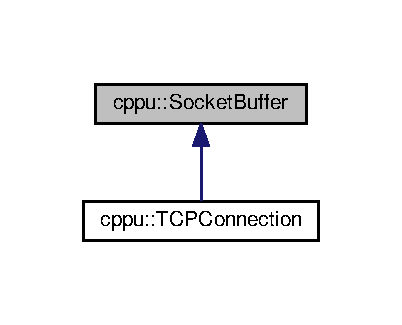
\includegraphics[width=193pt]{classcppu_1_1_socket_buffer__inherit__graph}
\end{center}
\end{figure}


Collaboration diagram for cppu\+:\+:Socket\+Buffer\+:
\nopagebreak
\begin{figure}[H]
\begin{center}
\leavevmode
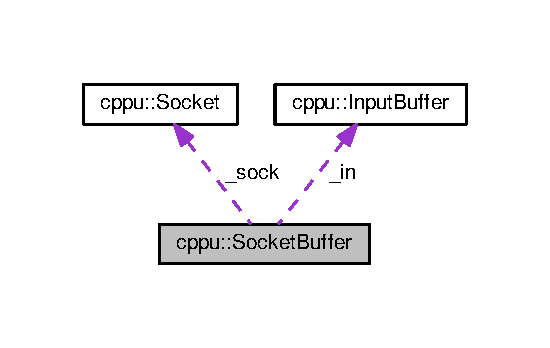
\includegraphics[width=264pt]{classcppu_1_1_socket_buffer__coll__graph}
\end{center}
\end{figure}
\subsection*{Public Member Functions}
\begin{DoxyCompactItemize}
\item 
\hypertarget{classcppu_1_1_socket_buffer_a1d6a8ae90bfcb69e6b3d2b9f97e3dc40}{\hyperlink{classcppu_1_1_socket_buffer_a1d6a8ae90bfcb69e6b3d2b9f97e3dc40}{Socket\+Buffer} (\hyperlink{classcppu_1_1_socket}{Socket} $\ast$\hyperlink{classcppu_1_1_socket_buffer_aab887b32ee999bfdd01c9a491c04bd61}{socket}, size\+\_\+t input\+Buffer\+Size=8192, size\+\_\+t ouput\+Buffer\+Size=8192)}\label{classcppu_1_1_socket_buffer_a1d6a8ae90bfcb69e6b3d2b9f97e3dc40}

\begin{DoxyCompactList}\small\item\em constructor. {\itshape socket} must be a connected T\+C\+P/\+I\+P \hyperlink{classcppu_1_1_socket}{Socket} (i.\+e. of S\+O\+C\+K\+\_\+\+S\+T\+R\+E\+A\+M type) that must {\itshape not} be deleted while the \hyperlink{classcppu_1_1_socket_buffer}{Socket\+Buffer} is used. {\itshape input\+Buffer\+Size} and {\itshape ouput\+Buffer\+Size} are the sizes of the buffers that used internally for exchanging the data. \end{DoxyCompactList}\item 
\hypertarget{classcppu_1_1_socket_buffer_ae8e387747f17f4ff3bfe036ccf11e89b}{{\bfseries Socket\+Buffer} (\hyperlink{classcppu_1_1_socket}{Socket} \&\hyperlink{classcppu_1_1_socket_buffer_aab887b32ee999bfdd01c9a491c04bd61}{socket}, size\+\_\+t input\+Buffer\+Size=8192, size\+\_\+t ouput\+Buffer\+Size=8192)}\label{classcppu_1_1_socket_buffer_ae8e387747f17f4ff3bfe036ccf11e89b}

\item 
\hypertarget{classcppu_1_1_socket_buffer_aab887b32ee999bfdd01c9a491c04bd61}{\hyperlink{classcppu_1_1_socket}{Socket} $\ast$ \hyperlink{classcppu_1_1_socket_buffer_aab887b32ee999bfdd01c9a491c04bd61}{socket} ()}\label{classcppu_1_1_socket_buffer_aab887b32ee999bfdd01c9a491c04bd61}

\begin{DoxyCompactList}\small\item\em returns the associated socket. \end{DoxyCompactList}\item 
\hypertarget{classcppu_1_1_socket_buffer_a77dfe31ad3d5660322d788daf213534e}{int \hyperlink{classcppu_1_1_socket_buffer_a77dfe31ad3d5660322d788daf213534e}{input\+Separator} () const }\label{classcppu_1_1_socket_buffer_a77dfe31ad3d5660322d788daf213534e}

\begin{DoxyCompactList}\small\item\em returns the input separator. \end{DoxyCompactList}\item 
\hypertarget{classcppu_1_1_socket_buffer_a737c72f4ce5ff73a2e7339430b6d1614}{int \hyperlink{classcppu_1_1_socket_buffer_a737c72f4ce5ff73a2e7339430b6d1614}{output\+Separator} () const }\label{classcppu_1_1_socket_buffer_a737c72f4ce5ff73a2e7339430b6d1614}

\begin{DoxyCompactList}\small\item\em returns the output separator. \end{DoxyCompactList}\item 
virtual void \hyperlink{classcppu_1_1_socket_buffer_acadf4540c1e3eba67b014753b84b482c}{set\+Input\+Separator} (int separ)
\begin{DoxyCompactList}\small\item\em changes the input separator. This function specifies the character(s) used by \hyperlink{classcppu_1_1_socket_buffer_a222769d3776b9cbd3a727ee1f0e60358}{read\+Line()} to separate successive lines\+: \end{DoxyCompactList}\item 
virtual void \hyperlink{classcppu_1_1_socket_buffer_a0e5e6a9ce3bda28b65c559c8b3c91b0f}{set\+Output\+Separator} (int separ)
\begin{DoxyCompactList}\small\item\em changes the output separator. This function specifies the character(s) used by \hyperlink{classcppu_1_1_socket_buffer_a92ae0351aaee8719d34e8c4618495d59}{write\+Line()} to separate successive lines\+: \end{DoxyCompactList}\item 
virtual ssize\+\_\+t \hyperlink{classcppu_1_1_socket_buffer_a222769d3776b9cbd3a727ee1f0e60358}{read\+Line} (std\+::string \&str)
\begin{DoxyCompactList}\small\item\em Reads a line of text from a connected socket. \hyperlink{classcppu_1_1_socket_buffer_a222769d3776b9cbd3a727ee1f0e60358}{read\+Line()} receives one line of text sent by \hyperlink{classcppu_1_1_socket_buffer_a92ae0351aaee8719d34e8c4618495d59}{write\+Line()} on the other side. The text is stored in {\itshape str}. This method blocks until the complete text line is received. \end{DoxyCompactList}\item 
virtual ssize\+\_\+t \hyperlink{classcppu_1_1_socket_buffer_a92ae0351aaee8719d34e8c4618495d59}{write\+Line} (const std\+::string \&str)
\begin{DoxyCompactList}\small\item\em Sends a line of text to a connected socket. \hyperlink{classcppu_1_1_socket_buffer_a92ae0351aaee8719d34e8c4618495d59}{write\+Line()} sends one line of text that will be received by a single call to \hyperlink{classcppu_1_1_socket_buffer_a222769d3776b9cbd3a727ee1f0e60358}{read\+Line()} on the other side (see note below). \end{DoxyCompactList}\item 
\hypertarget{classcppu_1_1_socket_buffer_a27de273ae2defbf3a5cc308310b9835e}{virtual ssize\+\_\+t {\bfseries read} (char $\ast$buffer, size\+\_\+t len)}\label{classcppu_1_1_socket_buffer_a27de273ae2defbf3a5cc308310b9835e}

\item 
\hypertarget{classcppu_1_1_socket_buffer_ab4ed032f329be2f6ecd0cba5fcd0518d}{virtual ssize\+\_\+t {\bfseries write} (const char $\ast$str, size\+\_\+t len)}\label{classcppu_1_1_socket_buffer_ab4ed032f329be2f6ecd0cba5fcd0518d}

\end{DoxyCompactItemize}
\subsection*{Protected Member Functions}
\begin{DoxyCompactItemize}
\item 
\hypertarget{classcppu_1_1_socket_buffer_ae634cbe12f6688a8d64c4579299e9802}{virtual bool {\bfseries retrieve\+Line} (std\+::string \&str, ssize\+\_\+t received)}\label{classcppu_1_1_socket_buffer_ae634cbe12f6688a8d64c4579299e9802}

\end{DoxyCompactItemize}
\subsection*{Protected Attributes}
\begin{DoxyCompactItemize}
\item 
\hypertarget{classcppu_1_1_socket_buffer_af52d0e7a5fb70ad371693c2e7f9f056b}{size\+\_\+t {\bfseries \+\_\+in\+Size}}\label{classcppu_1_1_socket_buffer_af52d0e7a5fb70ad371693c2e7f9f056b}

\item 
\hypertarget{classcppu_1_1_socket_buffer_afa2daeed2c8538030353382f48269896}{size\+\_\+t {\bfseries \+\_\+out\+Size}}\label{classcppu_1_1_socket_buffer_afa2daeed2c8538030353382f48269896}

\item 
\hypertarget{classcppu_1_1_socket_buffer_a5bf8f3a5ef56fc6f15ade71fe55b049d}{int {\bfseries \+\_\+in\+Sep}}\label{classcppu_1_1_socket_buffer_a5bf8f3a5ef56fc6f15ade71fe55b049d}

\item 
\hypertarget{classcppu_1_1_socket_buffer_a59b35cfa717476d18cc2e40c73073354}{int {\bfseries \+\_\+out\+Sep}}\label{classcppu_1_1_socket_buffer_a59b35cfa717476d18cc2e40c73073354}

\item 
\hypertarget{classcppu_1_1_socket_buffer_af60722acd94826d780bbb2477667d538}{\hyperlink{classcppu_1_1_socket}{Socket} $\ast$ {\bfseries \+\_\+sock}}\label{classcppu_1_1_socket_buffer_af60722acd94826d780bbb2477667d538}

\item 
\hypertarget{classcppu_1_1_socket_buffer_adb5986d6297496a1f92a30b1b3923072}{struct \hyperlink{structcppu_1_1_input_buffer}{Input\+Buffer} $\ast$ {\bfseries \+\_\+in}}\label{classcppu_1_1_socket_buffer_adb5986d6297496a1f92a30b1b3923072}

\end{DoxyCompactItemize}


\subsection{Detailed Description}
Preserves record boundaries when exchanging data between connected T\+C\+P/\+I\+P sockets. This class ensures that one call to \hyperlink{classcppu_1_1_socket_buffer_a92ae0351aaee8719d34e8c4618495d59}{write\+Line()} corresponds to one and exactly one call to \hyperlink{classcppu_1_1_socket_buffer_a222769d3776b9cbd3a727ee1f0e60358}{read\+Line()} on the other side. This differs from the behavior of \hyperlink{classcppu_1_1_socket_aeac77f859159715e2d63a5a0dc118788}{Socket\+::send()} and \hyperlink{classcppu_1_1_socket_a37c382af52cc02f92c0e19a0c6e0e04f}{Socket\+::receive()} because T\+C\+P/\+I\+P connected sockets do not preserve record boundaries. \hyperlink{classcppu_1_1_socket_buffer_a92ae0351aaee8719d34e8c4618495d59}{write\+Line()} and \hyperlink{classcppu_1_1_socket_buffer_a222769d3776b9cbd3a727ee1f0e60358}{read\+Line()} solve this problem by automatically adding and searching for a separator between successive lines. 

\begin{DoxySeeAlso}{See also}
\hyperlink{classcppu_1_1_socket_buffer_acadf4540c1e3eba67b014753b84b482c}{set\+Input\+Separator()} and \hyperlink{classcppu_1_1_socket_buffer_a0e5e6a9ce3bda28b65c559c8b3c91b0f}{set\+Output\+Separator()}. 
\end{DoxySeeAlso}


\subsection{Member Function Documentation}
\hypertarget{classcppu_1_1_socket_buffer_a222769d3776b9cbd3a727ee1f0e60358}{\index{cppu\+::\+Socket\+Buffer@{cppu\+::\+Socket\+Buffer}!read\+Line@{read\+Line}}
\index{read\+Line@{read\+Line}!cppu\+::\+Socket\+Buffer@{cppu\+::\+Socket\+Buffer}}
\subsubsection[{read\+Line}]{\setlength{\rightskip}{0pt plus 5cm}ssize\+\_\+t cppu\+::\+Socket\+Buffer\+::read\+Line (
\begin{DoxyParamCaption}
\item[{std\+::string \&}]{str}
\end{DoxyParamCaption}
)\hspace{0.3cm}{\ttfamily [virtual]}}}\label{classcppu_1_1_socket_buffer_a222769d3776b9cbd3a727ee1f0e60358}


Reads a line of text from a connected socket. \hyperlink{classcppu_1_1_socket_buffer_a222769d3776b9cbd3a727ee1f0e60358}{read\+Line()} receives one line of text sent by \hyperlink{classcppu_1_1_socket_buffer_a92ae0351aaee8719d34e8c4618495d59}{write\+Line()} on the other side. The text is stored in {\itshape str}. This method blocks until the complete text line is received. 

\hyperlink{classcppu_1_1_socket_buffer_a222769d3776b9cbd3a727ee1f0e60358}{read\+Line()} relies on a separator (by default, ~\newline
, ~\newline
 or ~\newline
, \begin{DoxySeeAlso}{See also}
\hyperlink{classcppu_1_1_socket_buffer_acadf4540c1e3eba67b014753b84b482c}{set\+Input\+Separator()}. This separator is automatically removed (it is not stored in {\itshape str}).
\end{DoxySeeAlso}
\begin{DoxyReturn}{Returns}
the number of bytes that were received or\+:
\begin{DoxyItemize}
\item 0\+: shutdown\+Output() was called on the other side
\item Socket\+::\+Failed (-\/1)\+: a connection error occured
\item Socket\+::\+Invalid\+Socket (-\/2)\+: the socket is invalid. The separator is counted in the value returned by \hyperlink{classcppu_1_1_socket_buffer_a222769d3776b9cbd3a727ee1f0e60358}{read\+Line()}. 
\end{DoxyItemize}
\end{DoxyReturn}
\hypertarget{classcppu_1_1_socket_buffer_acadf4540c1e3eba67b014753b84b482c}{\index{cppu\+::\+Socket\+Buffer@{cppu\+::\+Socket\+Buffer}!set\+Input\+Separator@{set\+Input\+Separator}}
\index{set\+Input\+Separator@{set\+Input\+Separator}!cppu\+::\+Socket\+Buffer@{cppu\+::\+Socket\+Buffer}}
\subsubsection[{set\+Input\+Separator}]{\setlength{\rightskip}{0pt plus 5cm}void cppu\+::\+Socket\+Buffer\+::set\+Input\+Separator (
\begin{DoxyParamCaption}
\item[{int}]{separ}
\end{DoxyParamCaption}
)\hspace{0.3cm}{\ttfamily [virtual]}}}\label{classcppu_1_1_socket_buffer_acadf4540c1e3eba67b014753b84b482c}


changes the input separator. This function specifies the character(s) used by \hyperlink{classcppu_1_1_socket_buffer_a222769d3776b9cbd3a727ee1f0e60358}{read\+Line()} to separate successive lines\+: 


\begin{DoxyItemize}
\item if {\itshape separ} $>$= 0, \hyperlink{classcppu_1_1_socket_buffer_a222769d3776b9cbd3a727ee1f0e60358}{read\+Line()} searches for {\itshape separ} to separate lines,
\item if {\itshape separ} $<$ 0, \hyperlink{classcppu_1_1_socket_buffer_a222769d3776b9cbd3a727ee1f0e60358}{read\+Line()} searches for ~\newline
,  or ~\newline
. By default, \hyperlink{classcppu_1_1_socket_buffer_a222769d3776b9cbd3a727ee1f0e60358}{read\+Line()} for ~\newline
,  or ~\newline
. \begin{DoxyNote}{Note}
If the input separator is changed, the output separator must be changed accordingly on the other side of the socket. 
\end{DoxyNote}
\begin{DoxySeeAlso}{See also}
\hyperlink{classcppu_1_1_socket_buffer_a0e5e6a9ce3bda28b65c559c8b3c91b0f}{set\+Output\+Separator()}. 
\end{DoxySeeAlso}

\end{DoxyItemize}\hypertarget{classcppu_1_1_socket_buffer_a0e5e6a9ce3bda28b65c559c8b3c91b0f}{\index{cppu\+::\+Socket\+Buffer@{cppu\+::\+Socket\+Buffer}!set\+Output\+Separator@{set\+Output\+Separator}}
\index{set\+Output\+Separator@{set\+Output\+Separator}!cppu\+::\+Socket\+Buffer@{cppu\+::\+Socket\+Buffer}}
\subsubsection[{set\+Output\+Separator}]{\setlength{\rightskip}{0pt plus 5cm}void cppu\+::\+Socket\+Buffer\+::set\+Output\+Separator (
\begin{DoxyParamCaption}
\item[{int}]{separ}
\end{DoxyParamCaption}
)\hspace{0.3cm}{\ttfamily [virtual]}}}\label{classcppu_1_1_socket_buffer_a0e5e6a9ce3bda28b65c559c8b3c91b0f}


changes the output separator. This function specifies the character(s) used by \hyperlink{classcppu_1_1_socket_buffer_a92ae0351aaee8719d34e8c4618495d59}{write\+Line()} to separate successive lines\+: 


\begin{DoxyItemize}
\item if {\itshape separ} $>$= 0, \hyperlink{classcppu_1_1_socket_buffer_a92ae0351aaee8719d34e8c4618495d59}{write\+Line()} inserts {\itshape separ} between successive lines,
\item if {\itshape separ} $<$ 0, \hyperlink{classcppu_1_1_socket_buffer_a92ae0351aaee8719d34e8c4618495d59}{write\+Line()} inserts ~\newline
 between successive lines. By default, \hyperlink{classcppu_1_1_socket_buffer_a92ae0351aaee8719d34e8c4618495d59}{write\+Line()} inserts ~\newline
. \begin{DoxyNote}{Note}
If the output separator is changed, the input separator must be changed accordingly on the other side of the socket. 
\end{DoxyNote}
\begin{DoxySeeAlso}{See also}
\hyperlink{classcppu_1_1_socket_buffer_acadf4540c1e3eba67b014753b84b482c}{set\+Input\+Separator()}. 
\end{DoxySeeAlso}

\end{DoxyItemize}\hypertarget{classcppu_1_1_socket_buffer_a92ae0351aaee8719d34e8c4618495d59}{\index{cppu\+::\+Socket\+Buffer@{cppu\+::\+Socket\+Buffer}!write\+Line@{write\+Line}}
\index{write\+Line@{write\+Line}!cppu\+::\+Socket\+Buffer@{cppu\+::\+Socket\+Buffer}}
\subsubsection[{write\+Line}]{\setlength{\rightskip}{0pt plus 5cm}ssize\+\_\+t cppu\+::\+Socket\+Buffer\+::write\+Line (
\begin{DoxyParamCaption}
\item[{const std\+::string \&}]{str}
\end{DoxyParamCaption}
)\hspace{0.3cm}{\ttfamily [virtual]}}}\label{classcppu_1_1_socket_buffer_a92ae0351aaee8719d34e8c4618495d59}


Sends a line of text to a connected socket. \hyperlink{classcppu_1_1_socket_buffer_a92ae0351aaee8719d34e8c4618495d59}{write\+Line()} sends one line of text that will be received by a single call to \hyperlink{classcppu_1_1_socket_buffer_a222769d3776b9cbd3a727ee1f0e60358}{read\+Line()} on the other side (see note below). 

\hyperlink{classcppu_1_1_socket_buffer_a92ae0351aaee8719d34e8c4618495d59}{write\+Line()} relies on a separator (~\newline
 by default, \begin{DoxySeeAlso}{See also}
\hyperlink{classcppu_1_1_socket_buffer_a0e5e6a9ce3bda28b65c559c8b3c91b0f}{set\+Output\+Separator()}) that is automatically inserted between successive lines ().
\end{DoxySeeAlso}
\begin{DoxyReturn}{Returns}
the number of bytes that were sent or\+:
\begin{DoxyItemize}
\item 0\+: shutdown\+Input() was called on the other side
\item Socket\+::\+Failed (-\/1)\+: a connection error occured
\item Socket\+::\+Invalid\+Socket (-\/2)\+: the socket is invalid. The separator is counted in the value returned by \hyperlink{classcppu_1_1_socket_buffer_a92ae0351aaee8719d34e8c4618495d59}{write\+Line()}.
\end{DoxyItemize}
\end{DoxyReturn}
\begin{DoxyNote}{Note}
if {\itshape str} constains occurences of the separator, \hyperlink{classcppu_1_1_socket_buffer_a222769d3776b9cbd3a727ee1f0e60358}{read\+Line()} will be called several times on the other side. 
\end{DoxyNote}


The documentation for this class was generated from the following files\+:\begin{DoxyCompactItemize}
\item 
/cal/homes/fouotsap/\+Desktop/\+Fouotsap\+\_\+\+Foukmeniok\+\_\+\+Alain/cpp/cppsocket.\+h\item 
/cal/homes/fouotsap/\+Desktop/\+Fouotsap\+\_\+\+Foukmeniok\+\_\+\+Alain/cpp/cppsocket.\+cpp\end{DoxyCompactItemize}

\hypertarget{classcppu_1_1_t_c_p_connection}{\section{cppu\+:\+:T\+C\+P\+Connection Class Reference}
\label{classcppu_1_1_t_c_p_connection}\index{cppu\+::\+T\+C\+P\+Connection@{cppu\+::\+T\+C\+P\+Connection}}
}


Connection with a given client. Each \hyperlink{classcppu_1_1_t_c_p_connection}{T\+C\+P\+Connection} uses a different thread.  




{\ttfamily \#include $<$tcpserver.\+h$>$}



Inherits \hyperlink{classcppu_1_1_socket_buffer}{cppu\+::\+Socket\+Buffer}.

\subsection*{Public Member Functions}
\begin{DoxyCompactItemize}
\item 
\hypertarget{classcppu_1_1_t_c_p_connection_a4186946c7c22e3c2cebe3a97aa78f5f7}{\hyperlink{classcppu_1_1_t_c_p_server}{T\+C\+P\+Server} \& {\bfseries server} ()}\label{classcppu_1_1_t_c_p_connection_a4186946c7c22e3c2cebe3a97aa78f5f7}

\item 
\hypertarget{classcppu_1_1_t_c_p_connection_a4663875b80fced790502880c72e6e672}{pthread\+\_\+t {\bfseries thread} ()}\label{classcppu_1_1_t_c_p_connection_a4663875b80fced790502880c72e6e672}

\end{DoxyCompactItemize}
\subsection*{Friends}
\begin{DoxyCompactItemize}
\item 
\hypertarget{classcppu_1_1_t_c_p_connection_ae4cfdb1814d91a8d28dadb49adda68f0}{class {\bfseries T\+C\+P\+Server}}\label{classcppu_1_1_t_c_p_connection_ae4cfdb1814d91a8d28dadb49adda68f0}

\end{DoxyCompactItemize}
\subsection*{Additional Inherited Members}


\subsection{Detailed Description}
Connection with a given client. Each \hyperlink{classcppu_1_1_t_c_p_connection}{T\+C\+P\+Connection} uses a different thread. 

The documentation for this class was generated from the following files\+:\begin{DoxyCompactItemize}
\item 
/cal/homes/fouotsap/inf224/tcpserver.\+h\item 
/cal/homes/fouotsap/inf224/tcpserver.\+cpp\end{DoxyCompactItemize}

\hypertarget{classcppu_1_1_t_c_p_lock}{\section{cppu\+:\+:T\+C\+P\+Lock Class Reference}
\label{classcppu_1_1_t_c_p_lock}\index{cppu\+::\+T\+C\+P\+Lock@{cppu\+::\+T\+C\+P\+Lock}}
}


Locks the server in read mode or in write mode. Must be created {\itshape in the stack} by the callback method.  




{\ttfamily \#include $<$tcpserver.\+h$>$}

\subsection*{Public Member Functions}
\begin{DoxyCompactItemize}
\item 
\hyperlink{classcppu_1_1_t_c_p_lock_ad9ff8205f334918a69746ef90f731877}{T\+C\+P\+Lock} (\hyperlink{classcppu_1_1_t_c_p_connection}{T\+C\+P\+Connection} \&cnx, bool write\+Mode=false)
\begin{DoxyCompactList}\small\item\em locks the server in {\itshape write} or {\itshape read} mode. In order to avoid concurrency problems between threads, the callback method ( \end{DoxyCompactList}\end{DoxyCompactItemize}


\subsection{Detailed Description}
Locks the server in read mode or in write mode. Must be created {\itshape in the stack} by the callback method. 

\subsection{Constructor \& Destructor Documentation}
\hypertarget{classcppu_1_1_t_c_p_lock_ad9ff8205f334918a69746ef90f731877}{\index{cppu\+::\+T\+C\+P\+Lock@{cppu\+::\+T\+C\+P\+Lock}!T\+C\+P\+Lock@{T\+C\+P\+Lock}}
\index{T\+C\+P\+Lock@{T\+C\+P\+Lock}!cppu\+::\+T\+C\+P\+Lock@{cppu\+::\+T\+C\+P\+Lock}}
\subsubsection[{T\+C\+P\+Lock}]{\setlength{\rightskip}{0pt plus 5cm}cppu\+::\+T\+C\+P\+Lock\+::\+T\+C\+P\+Lock (
\begin{DoxyParamCaption}
\item[{{\bf T\+C\+P\+Connection} \&}]{cnx, }
\item[{bool}]{write\+Mode = {\ttfamily false}}
\end{DoxyParamCaption}
)}}\label{classcppu_1_1_t_c_p_lock_ad9ff8205f334918a69746ef90f731877}


locks the server in {\itshape write} or {\itshape read} mode. In order to avoid concurrency problems between threads, the callback method ( 

\begin{DoxySeeAlso}{See also}
set\+Callback()) can create a \hyperlink{classcppu_1_1_t_c_p_lock}{T\+C\+P\+Lock} object {\itshape in the stack} before performing a computation.
\end{DoxySeeAlso}
{\itshape write\+Mode} must be true if the callback changes data and false (the default) otherwise. A write\+Mode lock blocks all other locks (and the corresponding threads) until the callback method returns. 

The documentation for this class was generated from the following files\+:\begin{DoxyCompactItemize}
\item 
/cal/homes/fouotsap/\+Desktop/\+Fouotsap\+\_\+\+Foukmeniok\+\_\+\+Alain/cpp/tcpserver.\+h\item 
/cal/homes/fouotsap/\+Desktop/\+Fouotsap\+\_\+\+Foukmeniok\+\_\+\+Alain/cpp/tcpserver.\+cpp\end{DoxyCompactItemize}

\hypertarget{classcppu_1_1_t_c_p_server}{\section{cppu\+:\+:T\+C\+P\+Server Class Reference}
\label{classcppu_1_1_t_c_p_server}\index{cppu\+::\+T\+C\+P\+Server@{cppu\+::\+T\+C\+P\+Server}}
}


T\+C\+P/\+I\+P I\+Pv4 server. The server supports T\+C\+P/\+I\+P A\+F\+\_\+\+I\+N\+E\+T connections (following the I\+Pv4 Internet protocol) with multiple clients. One thread is used per client.  




{\ttfamily \#include $<$tcpserver.\+h$>$}



Collaboration diagram for cppu\+:\+:T\+C\+P\+Server\+:
\nopagebreak
\begin{figure}[H]
\begin{center}
\leavevmode
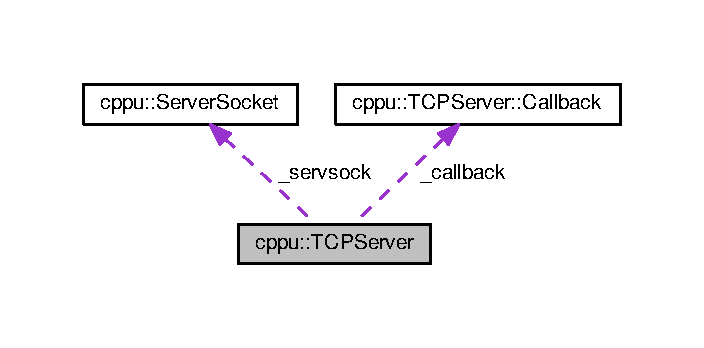
\includegraphics[width=338pt]{classcppu_1_1_t_c_p_server__coll__graph}
\end{center}
\end{figure}
\subsection*{Classes}
\begin{DoxyCompactItemize}
\item 
struct \hyperlink{structcppu_1_1_t_c_p_server_1_1_callback}{Callback}
\begin{DoxyCompactList}\small\item\em \hyperlink{structcppu_1_1_t_c_p_server_1_1_callback}{Callback} interface. \end{DoxyCompactList}\item 
struct \hyperlink{structcppu_1_1_t_c_p_server_1_1_callback_method}{Callback\+Method}
\end{DoxyCompactItemize}
\subsection*{Public Member Functions}
\begin{DoxyCompactItemize}
\item 
\hypertarget{classcppu_1_1_t_c_p_server_a48074f8409f580f6cf7b0be80200f9f3}{\hyperlink{classcppu_1_1_t_c_p_server_a48074f8409f580f6cf7b0be80200f9f3}{T\+C\+P\+Server} ()}\label{classcppu_1_1_t_c_p_server_a48074f8409f580f6cf7b0be80200f9f3}

\begin{DoxyCompactList}\small\item\em constructor\+: initializes the \hyperlink{classcppu_1_1_t_c_p_server}{T\+C\+P\+Server}. \end{DoxyCompactList}\item 
\hypertarget{classcppu_1_1_t_c_p_server_ababd20111e0cf4e14396433e56ca086e}{virtual \hyperlink{classcppu_1_1_t_c_p_server_ababd20111e0cf4e14396433e56ca086e}{$\sim$\+T\+C\+P\+Server} ()}\label{classcppu_1_1_t_c_p_server_ababd20111e0cf4e14396433e56ca086e}

\begin{DoxyCompactList}\small\item\em destructor\+: cleans up the \hyperlink{classcppu_1_1_t_c_p_server}{T\+C\+P\+Server}. \end{DoxyCompactList}\item 
virtual int \hyperlink{classcppu_1_1_t_c_p_server_a98e00d62745812b17bdee9f07f2070c4}{run} (int port)
\begin{DoxyCompactList}\small\item\em starts the \hyperlink{classcppu_1_1_t_c_p_server}{T\+C\+P\+Server}. \hyperlink{classcppu_1_1_t_c_p_server_a98e00d62745812b17bdee9f07f2070c4}{run()} binds an internal \hyperlink{classcppu_1_1_server_socket}{Server\+Socket} to {\itshape port} then starts an infinite loop that processes connection requests from clients. \end{DoxyCompactList}\item 
{\footnotesize template$<$class T $>$ }\\void \hyperlink{classcppu_1_1_t_c_p_server_a7d4fdb93439015934004755fde72945b}{set\+Callback} (T \&object, bool(T\+::$\ast$method)(\hyperlink{classcppu_1_1_t_c_p_connection}{T\+C\+P\+Connection} \&cnx, const std\+::string \&request, std\+::string \&response))
\begin{DoxyCompactList}\small\item\em changes the callback method of the \hyperlink{classcppu_1_1_t_c_p_server}{T\+C\+P\+Server}. This callback is called each time the \hyperlink{classcppu_1_1_t_c_p_server}{T\+C\+P\+Server} receives a request from a client. It can be any method of {\itshape object} with the following parameters\+: \end{DoxyCompactList}\item 
void \hyperlink{classcppu_1_1_t_c_p_server_a94d3d97b03d5e3e48609e405d8dd7897}{set\+Callback} (\hyperlink{structcppu_1_1_t_c_p_server_1_1_callback}{Callback} \&callback)
\begin{DoxyCompactList}\small\item\em changes the callback object of the \hyperlink{classcppu_1_1_t_c_p_server}{T\+C\+P\+Server}. \end{DoxyCompactList}\item 
\hypertarget{classcppu_1_1_t_c_p_server_a6428b63a4440045050dba4f33bb454bf}{\hyperlink{classcppu_1_1_server_socket}{Server\+Socket} \& \hyperlink{classcppu_1_1_t_c_p_server_a6428b63a4440045050dba4f33bb454bf}{server\+Socket} ()}\label{classcppu_1_1_t_c_p_server_a6428b63a4440045050dba4f33bb454bf}

\begin{DoxyCompactList}\small\item\em returns the internal \hyperlink{classcppu_1_1_server_socket}{Server\+Socket}. \end{DoxyCompactList}\item 
\hypertarget{classcppu_1_1_t_c_p_server_afc47ca4476d9c75d5ea88f73e2acd6d5}{virtual void \hyperlink{classcppu_1_1_t_c_p_server_afc47ca4476d9c75d5ea88f73e2acd6d5}{error} (const std\+::string \&msg, const \hyperlink{classcppu_1_1_t_c_p_connection}{T\+C\+P\+Connection} $\ast$=nullptr)}\label{classcppu_1_1_t_c_p_server_afc47ca4476d9c75d5ea88f73e2acd6d5}

\begin{DoxyCompactList}\small\item\em prints warning and error messages on the terminal. \end{DoxyCompactList}\end{DoxyCompactItemize}
\subsection*{Protected Member Functions}
\begin{DoxyCompactItemize}
\item 
\hypertarget{classcppu_1_1_t_c_p_server_abe314b95a31c88b479c81ec9bf123c65}{virtual \hyperlink{classcppu_1_1_t_c_p_connection}{T\+C\+P\+Connection} $\ast$ \hyperlink{classcppu_1_1_t_c_p_server_abe314b95a31c88b479c81ec9bf123c65}{create\+Cnx} (\hyperlink{classcppu_1_1_socket}{Socket} $\ast$)}\label{classcppu_1_1_t_c_p_server_abe314b95a31c88b479c81ec9bf123c65}

\begin{DoxyCompactList}\small\item\em creates a new connection that starts a new thread for listening this socket. \end{DoxyCompactList}\end{DoxyCompactItemize}
\subsection*{Protected Attributes}
\begin{DoxyCompactItemize}
\item 
\hypertarget{classcppu_1_1_t_c_p_server_a8e4422abf23dc5bd195d05a3e9eee167}{\hyperlink{classcppu_1_1_server_socket}{Server\+Socket} {\bfseries \+\_\+servsock}}\label{classcppu_1_1_t_c_p_server_a8e4422abf23dc5bd195d05a3e9eee167}

\item 
\hypertarget{classcppu_1_1_t_c_p_server_abe36d427d7b047cdd342e282611c841e}{std\+::shared\+\_\+ptr$<$ \hyperlink{structcppu_1_1_t_c_p_server_1_1_callback}{Callback} $>$ {\bfseries \+\_\+callback\+Ptr}}\label{classcppu_1_1_t_c_p_server_abe36d427d7b047cdd342e282611c841e}

\item 
\hypertarget{classcppu_1_1_t_c_p_server_a68940bd70ac6941ca49d1e51b631f5e9}{\hyperlink{structcppu_1_1_t_c_p_server_1_1_callback}{Callback} $\ast$ {\bfseries \+\_\+callback}}\label{classcppu_1_1_t_c_p_server_a68940bd70ac6941ca49d1e51b631f5e9}

\item 
\hypertarget{classcppu_1_1_t_c_p_server_aea2dbb4b5762044217096e52cd559b97}{pthread\+\_\+rwlock\+\_\+t {\bfseries \+\_\+threadlock}}\label{classcppu_1_1_t_c_p_server_aea2dbb4b5762044217096e52cd559b97}

\end{DoxyCompactItemize}
\subsection*{Friends}
\begin{DoxyCompactItemize}
\item 
\hypertarget{classcppu_1_1_t_c_p_server_a94abdeb80587f39a869fde6f24522a78}{class {\bfseries T\+C\+P\+Lock}}\label{classcppu_1_1_t_c_p_server_a94abdeb80587f39a869fde6f24522a78}

\item 
\hypertarget{classcppu_1_1_t_c_p_server_a9d1c27bdfcdd48c5f07a5d0dce43b346}{class {\bfseries T\+C\+P\+Connection}}\label{classcppu_1_1_t_c_p_server_a9d1c27bdfcdd48c5f07a5d0dce43b346}

\end{DoxyCompactItemize}


\subsection{Detailed Description}
T\+C\+P/\+I\+P I\+Pv4 server. The server supports T\+C\+P/\+I\+P A\+F\+\_\+\+I\+N\+E\+T connections (following the I\+Pv4 Internet protocol) with multiple clients. One thread is used per client. 

Call \hyperlink{classcppu_1_1_t_c_p_server_a7d4fdb93439015934004755fde72945b}{set\+Callback()} to specify the callback method that will be invoked each time a request is sent by a client then \hyperlink{classcppu_1_1_t_c_p_server_a98e00d62745812b17bdee9f07f2070c4}{run()} to start the server.

Requests can be processed concurrently thanks to threads. To avoid concurrency problems the callback can perform a read or write lock (\begin{DoxySeeAlso}{See also}
\hyperlink{classcppu_1_1_t_c_p_lock}{T\+C\+P\+Lock}). 
\end{DoxySeeAlso}


\subsection{Member Function Documentation}
\hypertarget{classcppu_1_1_t_c_p_server_a98e00d62745812b17bdee9f07f2070c4}{\index{cppu\+::\+T\+C\+P\+Server@{cppu\+::\+T\+C\+P\+Server}!run@{run}}
\index{run@{run}!cppu\+::\+T\+C\+P\+Server@{cppu\+::\+T\+C\+P\+Server}}
\subsubsection[{run}]{\setlength{\rightskip}{0pt plus 5cm}int cppu\+::\+T\+C\+P\+Server\+::run (
\begin{DoxyParamCaption}
\item[{int}]{port}
\end{DoxyParamCaption}
)\hspace{0.3cm}{\ttfamily [virtual]}}}\label{classcppu_1_1_t_c_p_server_a98e00d62745812b17bdee9f07f2070c4}


starts the \hyperlink{classcppu_1_1_t_c_p_server}{T\+C\+P\+Server}. \hyperlink{classcppu_1_1_t_c_p_server_a98e00d62745812b17bdee9f07f2070c4}{run()} binds an internal \hyperlink{classcppu_1_1_server_socket}{Server\+Socket} to {\itshape port} then starts an infinite loop that processes connection requests from clients. 

For each successful connection request, a \hyperlink{classcppu_1_1_t_c_p_connection}{T\+C\+P\+Connection} object is created. This object starts a thread that processes incoming requests from its client. A callback method (\begin{DoxySeeAlso}{See also}
\hyperlink{classcppu_1_1_t_c_p_server_a7d4fdb93439015934004755fde72945b}{set\+Callback()}) is invoked for each request.
\end{DoxySeeAlso}
\begin{DoxyReturn}{Returns}
0 on normal termination or a negative value if the \hyperlink{classcppu_1_1_server_socket}{Server\+Socket} could not be bound (value is then one of \hyperlink{classcppu_1_1_socket_a49ea5cb079bd7ae97ecf7eb30c9d9e5f}{Socket\+::\+Errors}). 
\end{DoxyReturn}
\hypertarget{classcppu_1_1_t_c_p_server_a7d4fdb93439015934004755fde72945b}{\index{cppu\+::\+T\+C\+P\+Server@{cppu\+::\+T\+C\+P\+Server}!set\+Callback@{set\+Callback}}
\index{set\+Callback@{set\+Callback}!cppu\+::\+T\+C\+P\+Server@{cppu\+::\+T\+C\+P\+Server}}
\subsubsection[{set\+Callback}]{\setlength{\rightskip}{0pt plus 5cm}template$<$class T $>$ void cppu\+::\+T\+C\+P\+Server\+::set\+Callback (
\begin{DoxyParamCaption}
\item[{T \&}]{object, }
\item[{bool(T\+::$\ast$)({\bf T\+C\+P\+Connection} \&cnx, const std\+::string \&request, std\+::string \&response)}]{method}
\end{DoxyParamCaption}
)\hspace{0.3cm}{\ttfamily [inline]}}}\label{classcppu_1_1_t_c_p_server_a7d4fdb93439015934004755fde72945b}


changes the callback method of the \hyperlink{classcppu_1_1_t_c_p_server}{T\+C\+P\+Server}. This callback is called each time the \hyperlink{classcppu_1_1_t_c_p_server}{T\+C\+P\+Server} receives a request from a client. It can be any method of {\itshape object} with the following parameters\+: 


\begin{DoxyItemize}
\item {\itshape cnx} is the connection with the client sending the request
\item {\itshape request} contains the data sent by the client
\item {\itshape response} will be sent to the client as a response The connection is closed if the callback returns false.
\end{DoxyItemize}

To avoid concurrency problems, the callback should perform a read or write lock (\begin{DoxySeeAlso}{See also}
\hyperlink{classcppu_1_1_t_c_p_lock}{T\+C\+P\+Lock}) before performing a computation. 
\end{DoxySeeAlso}
\hypertarget{classcppu_1_1_t_c_p_server_a94d3d97b03d5e3e48609e405d8dd7897}{\index{cppu\+::\+T\+C\+P\+Server@{cppu\+::\+T\+C\+P\+Server}!set\+Callback@{set\+Callback}}
\index{set\+Callback@{set\+Callback}!cppu\+::\+T\+C\+P\+Server@{cppu\+::\+T\+C\+P\+Server}}
\subsubsection[{set\+Callback}]{\setlength{\rightskip}{0pt plus 5cm}void cppu\+::\+T\+C\+P\+Server\+::set\+Callback (
\begin{DoxyParamCaption}
\item[{{\bf Callback} \&}]{callback}
\end{DoxyParamCaption}
)\hspace{0.3cm}{\ttfamily [inline]}}}\label{classcppu_1_1_t_c_p_server_a94d3d97b03d5e3e48609e405d8dd7897}


changes the callback object of the \hyperlink{classcppu_1_1_t_c_p_server}{T\+C\+P\+Server}. 

\begin{DoxySeeAlso}{See also}
set\+Callback(object, method). 
\end{DoxySeeAlso}


The documentation for this class was generated from the following files\+:\begin{DoxyCompactItemize}
\item 
/cal/homes/fouotsap/\+Desktop/\+Fouotsap\+\_\+\+Foukmeniok\+\_\+\+Alain/cpp/tcpserver.\+h\item 
/cal/homes/fouotsap/\+Desktop/\+Fouotsap\+\_\+\+Foukmeniok\+\_\+\+Alain/cpp/tcpserver.\+cpp\end{DoxyCompactItemize}

\hypertarget{class_video}{\section{Video Class Reference}
\label{class_video}\index{Video@{Video}}
}


Inherits \hyperlink{class_omultimedia}{Omultimedia}.



Inherited by \hyperlink{class_film}{Film}.

\subsection*{Public Member Functions}
\begin{DoxyCompactItemize}
\item 
\hypertarget{class_video_a5d535758640a431850f8d67773b20211}{{\bfseries Video} (unsigned int duree, string nom\+Video, string nom\+Path\+Video)}\label{class_video_a5d535758640a431850f8d67773b20211}

\item 
\hypertarget{class_video_ac9ed820535234a8c6520f68a60e72a61}{unsigned int {\bfseries get\+Duree} () const }\label{class_video_ac9ed820535234a8c6520f68a60e72a61}

\item 
\hypertarget{class_video_a8174feb6113c5b55a38b138d5be3e97b}{void {\bfseries set\+Duree} (unsigned int duree)}\label{class_video_a8174feb6113c5b55a38b138d5be3e97b}

\item 
void \hyperlink{class_video_a3a4dd11a3021cf824d98006498d0b2af}{afficher\+Objet} (ostream \&s) const override
\begin{DoxyCompactList}\small\item\em \hyperlink{class_video_a3a4dd11a3021cf824d98006498d0b2af}{Video\+::afficher\+Objet}. \end{DoxyCompactList}\item 
void \hyperlink{class_video_a62e160d1dc506f032841f2763c8e9377}{jouer\+Objet} (string nom\+Objet, string path) const override
\begin{DoxyCompactList}\small\item\em \hyperlink{class_video_a62e160d1dc506f032841f2763c8e9377}{Video\+::jouer\+Objet}. \end{DoxyCompactList}\end{DoxyCompactItemize}


\subsection{Member Function Documentation}
\hypertarget{class_video_a3a4dd11a3021cf824d98006498d0b2af}{\index{Video@{Video}!afficher\+Objet@{afficher\+Objet}}
\index{afficher\+Objet@{afficher\+Objet}!Video@{Video}}
\subsubsection[{afficher\+Objet}]{\setlength{\rightskip}{0pt plus 5cm}void Video\+::afficher\+Objet (
\begin{DoxyParamCaption}
\item[{ostream \&}]{s}
\end{DoxyParamCaption}
) const\hspace{0.3cm}{\ttfamily [override]}, {\ttfamily [virtual]}}}\label{class_video_a3a4dd11a3021cf824d98006498d0b2af}


\hyperlink{class_video_a3a4dd11a3021cf824d98006498d0b2af}{Video\+::afficher\+Objet}. 


\begin{DoxyParams}{Parameters}
{\em s} & \\
\hline
\end{DoxyParams}


Implements \hyperlink{class_omultimedia_ae8942bb1db61d92962a71bbe7512c037}{Omultimedia}.

\hypertarget{class_video_a62e160d1dc506f032841f2763c8e9377}{\index{Video@{Video}!jouer\+Objet@{jouer\+Objet}}
\index{jouer\+Objet@{jouer\+Objet}!Video@{Video}}
\subsubsection[{jouer\+Objet}]{\setlength{\rightskip}{0pt plus 5cm}void Video\+::jouer\+Objet (
\begin{DoxyParamCaption}
\item[{string}]{nom\+Objet, }
\item[{string}]{path}
\end{DoxyParamCaption}
) const\hspace{0.3cm}{\ttfamily [override]}, {\ttfamily [virtual]}}}\label{class_video_a62e160d1dc506f032841f2763c8e9377}


\hyperlink{class_video_a62e160d1dc506f032841f2763c8e9377}{Video\+::jouer\+Objet}. 


\begin{DoxyParams}{Parameters}
{\em nom\+Objet} & \+: Nom de l'objet à jouer. Nom photo ou nom de la video \\
\hline
{\em path} & emplacement de l'objet \\
\hline
\end{DoxyParams}


Implements \hyperlink{class_omultimedia}{Omultimedia}.



The documentation for this class was generated from the following files\+:\begin{DoxyCompactItemize}
\item 
/cal/homes/fouotsap/inf224/Video.\+h\item 
/cal/homes/fouotsap/inf224/Video.\+cpp\end{DoxyCompactItemize}

%--- End generated contents ---

% Index
\newpage
\phantomsection
\addcontentsline{toc}{chapter}{Index}
\printindex

\end{document}
